\documentclass{article}
\usepackage{float}
\usepackage{graphicx}
\usepackage{cancel}
\usepackage{amsmath}
\usepackage[includehead,nomarginpar]{geometry}
\usepackage[export]{adjustbox}
\usepackage{amsfonts} 
\usepackage{verbatim}
\usepackage{mathrsfs}  
\usepackage{lmodern}
\usepackage{bm}
\usepackage{braket}
\usepackage{bookmark}
\usepackage[italian]{babel}
\usepackage{fancyhdr}
\usepackage{romanbarpagenumber}
\usepackage{subcaption}
\usepackage{caption}
\usepackage{float}
\usepackage[export]{adjustbox}
\usepackage{bm}
\usepackage{lipsum}
\usepackage{capt-of}
\usepackage{tikz}
\usepackage{xcolor}
\allowdisplaybreaks

\setlength{\headheight}{12.0pt}
\addtolength{\topmargin}{-12.0pt}
\graphicspath{ {./Immagini/} }



%% segnati con un doppio segno percentuale ("%%") le correzioni o inserimenti da apportare al testo  


\hypersetup{
    colorlinks=true,
    linkcolor=black,
}

\renewcommand{\contentsname}{Indice}
\AtBeginDocument{%
  \renewcommand{\figurename}{Fig.}
}
\newcommand{\vect}[1]{\boldsymbol{\mathbf{#1}}}
\newcommand{\df}{\mathrm{d}}
\newcommand{\Frac}[2]{\displaystyle\frac{\strut{#1}}{\strut{#2}}}
\newcommand{\tageq}{\tag{\stepcounter{equation}\theequation}}
\newcommand{\SI}[1]{\mathrm{#1}}


\newsavebox{\tempbox} %{\raisebox{\dimexpr.5\ht\tempbox-.5\height\relax}}


\numberwithin{equation}{subsection}

\begin{document}

\title{%
    \textbf{Fisica I Ripetizioni Parte 2}  \\ 
    \large Appunti delle ripetizioni di Fisica I Seconda Parte\\
    \textit{Anno Accademico: 2024/25}}
\author{\textit{Mattia Cosimi}}
\date{\textit{Dipartimento di Ingegneria Civile, Informatica e delle Tecnologie Aeronautiche \\
Università degli Studi ``Roma Tre"}}

\maketitle


\clearpage

\pagestyle{fancy}
\fancyhead{}\fancyfoot{}
\fancyhead[C]{\textit{Fisica I Ripetizioni Parte 2, Cosimi Mattia - Università degli Studi ``Roma Tre"}}
\fancyfoot[C]{\thepage}

\pagenumbering{Roman}
\tableofcontents

\clearpage

\pagenumbering{arabic}
\section{Lezione 11}
\subsection{Introduzione}
Iniziamo la parte di \textbf{termodinamica} che è quella scienza che \textbf{studia i passaggi di calore e di lavoro}.
\subsection{Principio 0 della termodinamica}
Il principio 0 della termodinamica ci dice che: due corpi che hanno diversa temperatura, si passano calore (energia in transito), il corpo più caldo passa calore al corpo più freddo fino a che i corpi non si posizionano in una \textbf{temperatura di equilibrio}. Raggiunto l'equilibrio non c'è più passaggio di calore e quindi anche corpi che hanno la stessa temperatura non si passano calore. Generalmente il passaggio di calore che consideriamo in fisica I è di tipo \textbf{conduttorio}: i due corpi sono in contatto.
\subsubsection{Corpi solidi, liquidi e gassosi}
Nei passaggi di calore vi è una differenza di temperatura in particolare:
\begin{itemize}
    \item se i corpi sono solidi rimangono costanti \textbf{volume e forma}
    \item se i corpi sono liquidi o liquido-solido, rimangono costanti volume e forma (data dal contenitore)
    \item se i corpi sono aeroformi (gassosi) le molecole che compongono il gas possono traslare tra di loro e il volume non rimane costante.
\end{itemize}
\noindent
I primi due vengono detti \textbf{incompressibili}, l'ultimo viene detto \textbf{compressibile} e quindi il gas si può espandere e comprimere grazie ai passaggi di calore. Questa proprietà è importante e ci aiuta con la scoperta delle \textbf{macchine termiche}.
\subsubsection{Macchine Termiche}
\begin{figure}[H]
    \centering
    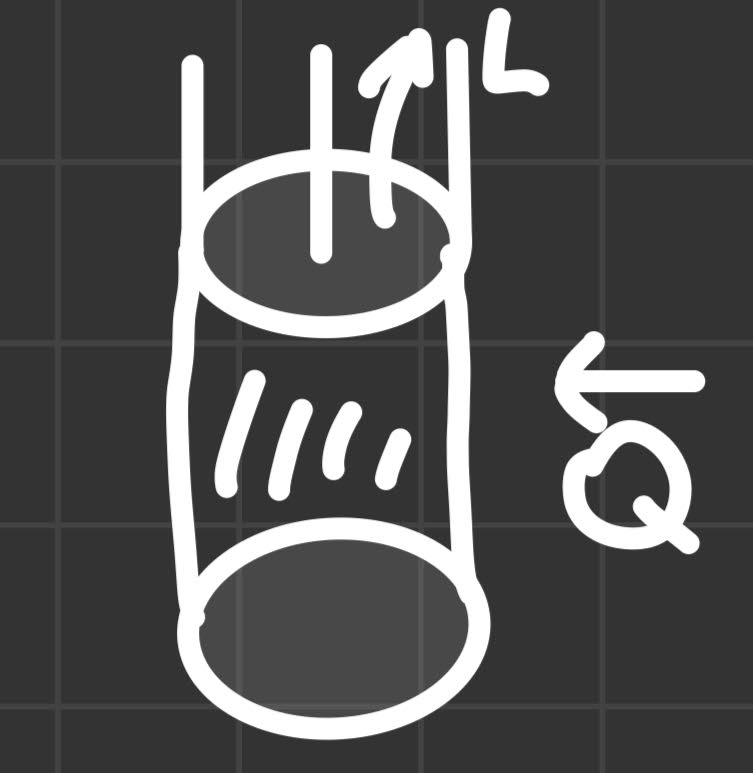
\includegraphics[width=0.2\linewidth]{MacchinaTermica.jpg}
    \label{fig:placeholder}
\end{figure}
\noindent
Schematizziamo una macchina termica in questo modo. Viene immesso del \textbf{calore} che entra nel gas, sopra a questo "cilindro" vi è un pistone da cui esce \textbf{lavoro}. Praticamente cosa succede: Il pistone fa in modo che il volume occupato dal gas sia quello proprio del gas e quest'ultimo si può comprimere o decomprimere. Le molecole con il calore prendono volume maggiore, il pistone tenderà quindi ad alzarsi, questo porta a pensare che ci sia una forza che lo sta alzando e questa è proprio la \textbf{pressione}. Il gas esprime lavoro verso l'esterno dato che comunque c'è una forza che sta compiendo uno spostamento. Il pistone quindi è utilizzabile per produrre lavoro e la chiave è proprio questa da calore passiamo a lavoro meccanico e questo nel corso della storia per l'uomo è stato molto importante. Infatti con i solidi, questo non è possibile dato che non c'è cambiamento di volume. Parliamo quindi di gerarchia delle fonti energetiche.
\subsection{Sistema Termodinamico}
Parliamo di sistema termodinamico, intendendo un corpo o un insieme di corpi che viene studiato dal punto di vista delle variabili termodinamiche, le quali variano al variare di calore e lavoro. Queste variabili sono: \textbf{la temperatura}, la quale cambia nel passaggio di calore, \textbf{il volume}, il quale non cambia in liquidi e solidi ma cambia nei gas e \textbf{la pressione} la quale cambia con il calore, l'insieme di queste tre definisce lo \textbf{stato termodinamico}. Dato che lo stato termodinamico varia voglio rappresentarlo in maniera sintetica, potrei pensare di rappresentarlo con un punto presi tre assi nello spazio cartesiano, in realtà cerco una rappresentazione più semplice per rappresentarlo nel piano bidimensionale. Per farlo ho bisogno di rappresentare 2 variabili termodinamiche e avere una variabile in funzione dell'altra. Questo legame è dato da:
\subsubsection{Equazione di stato dei gas perfetti}
Parliamo di stato perchè questa vale in ogni istante di tempo e stato sta per stato termodinamico. C'è da dire che in realtà ci sarebbero illimitate equazioni di stato a seconda della specie tipo del gas, si è allora trovata quest'equazione che vale più o meno per tutti, infatti si è preso un gas perfetto che si avvicina alla realtà.
\begin{equation}
    PV=nRT
\end{equation}
Dove la P sta per \textbf{pressione}, la V sta per \textbf{volume}, la n sta per \textbf{numero di moli}, la T sta per \textbf{temperatura} e la R sta per \textbf{costante universale di gas}. Apriamo una parentesi relativa agli esercizi per la R, questa ha alcuni valori possibili i quali dipendono dalle unità di misura di PVT, utilizziamo allora un solo valore $R=8.3$ a patto di utilizzare sempre queste unità di misura:
\begin{equation}
    P=Pascal \  (Pa) \ \ \ \ T=Kelvin \ (K) \ \ \ \ V=m^3
\end{equation}
Bisogna quindi imparare le conversioni, la pressione può anche essere espressa in bar o atmosfere (per le quali vale la stessa conversione), la temperatura può essere espressa in gradi celsius, il volume in decine di cubi o litri (per i quali vale la stessa conversione):
\begin{align}
    & 1 \ bar=10^5 \ Pa \ \ \ \ es. \ \ 0.3 \ bar=30 000 \ Pa \\
    & 1 {}^{\circ}C = 1 + 273 \ K \\
    & 1 \ l = 10^{-3} m^3
\end{align}
Definita questa allora possiamo vedere come rappresentare lo \textbf{stato termodinamico}.
\subsubsection{Piano di Clapeyron (PV)}
\begin{figure}[H]
    \centering
    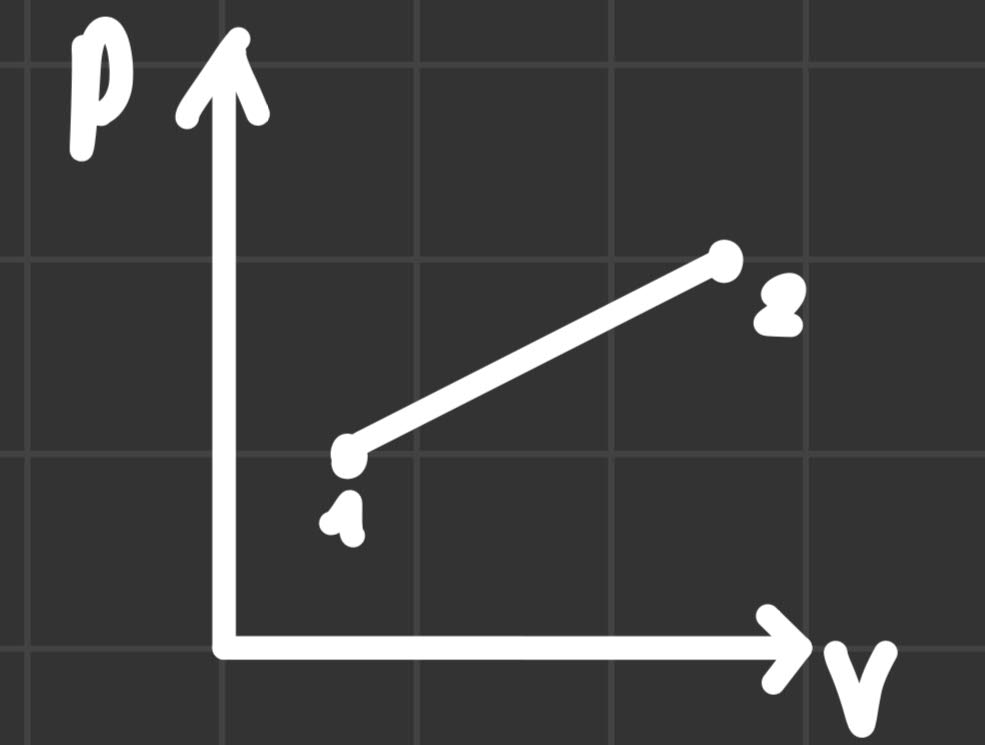
\includegraphics[width=0.3\linewidth]{PianoDiClapeyron.jpg}
    \label{fig:placeholder}
\end{figure}
\noindent
Il tratto e quindi la traiettoria viene detta \textbf{trasformazione termodinamica}, ci permette di rappresentare l'inizio e la fine dello stato termodinamico. Ovviamente questa traiettoria dipende da quanto calore e lavoro gli do. Se prendiamo inizio e fine di ogni trasformazione e tracciamo le verticali, otterremo un area sottesa (integrale) che corrisponde al \textbf{lavoro della trasformazione}.
\subsection{Trasformazioni Termodinamiche}
Le macchine termiche nella storia sono state utilizzate nelle industrie. Per questo motivo le trasformazioni che applico ho bisogno che siano compatibili a più macchine possibile utilizzando le stesse tecnologie anche andando a risparmio economico. Quindi devono essere standardizzate tecnologicamente e facili da effettuare, facili anche dal punto di vista del calcolo. Sono 4 le trasformazioni dei cicli a cui sono soggetti i gas nelle macchine termiche. Nota: ogni trasformazione ha una \textbf{legge di trasformazione} la quale ci consente di calcolare le variabili termodinamiche di inizio o fine.
\subsubsection{Isocora}
Nella trasformazione \textbf{isocora} rimane costante il volume dei gas. Per cui la sua rappresentazione sul piano di Claperyron sarà:
\begin{figure}[H]
    \centering
    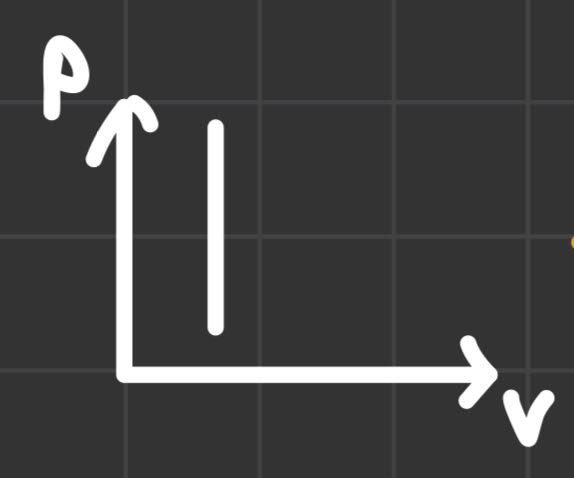
\includegraphics[width=0.25\linewidth]{Isocora.jpg}
    \label{fig:placeholder}
\end{figure}
\noindent
La sua legge di trasformazione viene detta \textbf{legge di Gaylussac} e ci dice che lungo un isocora si mantiene costante il rapporto $\frac{P}{T}$:
\begin{equation}
    \frac{P_i}{T_i}=\frac{P_f}{T_f}
\end{equation}
Nota: negli esercizi non avremo mai tre incognite e calcolo semplicemente la quarta, motivo per il quale ho bisogno di altre equazioni. In tutte le trasformazioni a eccezione dell'adiabatica, vi è passaggio di calore il quale ha sempre la stessa sintassi:
\begin{equation}
    Q=nc\Delta T
\end{equation}
Dove Q appunto è il \textbf{calore}, n è il \textbf{numero di moli}, c è il \textbf{calore specifico della trasformazione} e $\Delta T$ è la variazione di temperatura. Quindi nell'isocora avremo \textbf{calore specifico a volume costante}.
\begin{equation}
    Q=nc_V\Delta T
\end{equation}
Essendo il volume costante in questa trasformazione il lavoro è nullo $W=0$. Basti vedere che tracciando le verticali, non vi è area sottesa.
\subsubsection{Isobara}
Nella trasformazione isobara vi si mantiene costante la pressione, per cui la sua rappresentazione sarà:
\begin{figure}[H]
    \centering
    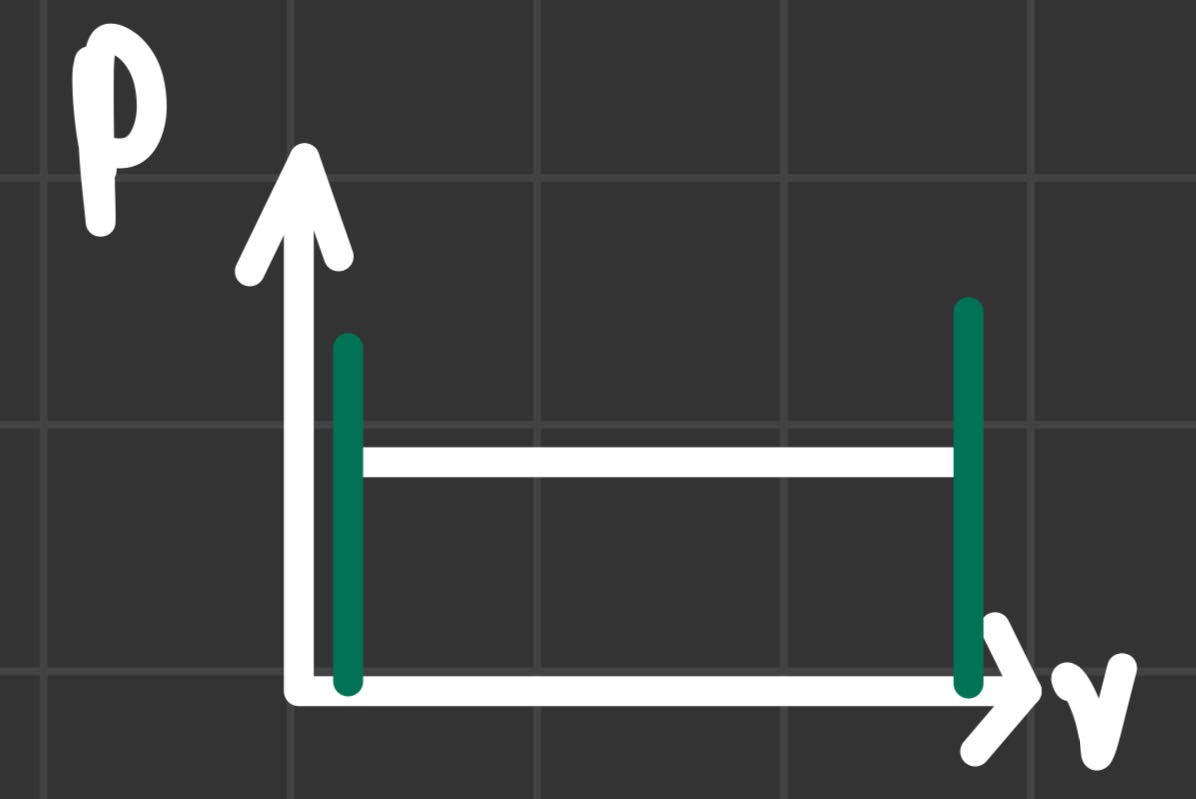
\includegraphics[width=0.25\linewidth]{Isobara.jpg}
    \label{fig:placeholder}
\end{figure}
\noindent
Come legge di trasformazione abbiamo la \textbf{seconda legge di Gaylussac} che ci dice che rimane costante il rapporto tra il volume e la temperatura:
\begin{equation}
    \frac{V_i}{T_i}=\frac{V_f}{T_f}
\end{equation}
Per il calore invece:
\begin{equation}
    Q=nc_P\Delta T
\end{equation}
Dove $c_P$ è il \textbf{calore specifico a pressione costante}. Per quanto riguarda il \textbf{lavoro}, tracciando le verticali notiamo che si viene a creare un rettangolo la cui area è $b*h$ abbiamo quindi:
\begin{equation}
    W= \Delta V * P
\end{equation}
Dove $\Delta V$ è la variazione di volume. 
\newpage
\subsubsection{Isoterma}
Nella trasformazione isoterma si mantiene costante la temperatura la sua rappresentazione sul piano di Gaylussac:
\begin{figure}[H]
    \centering
    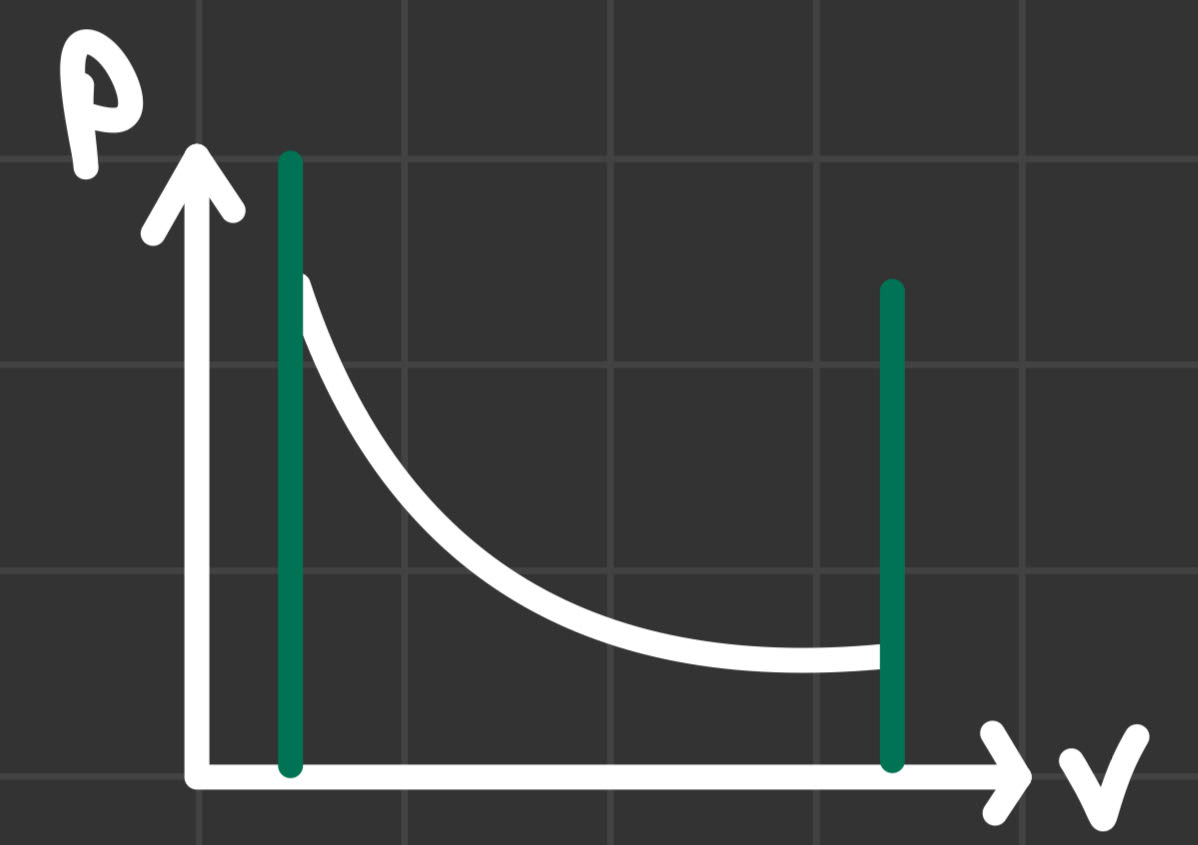
\includegraphics[width=0.25\linewidth]{IsoTerma.jpg}
    \label{fig:placeholder}
\end{figure}
\noindent
Risulta essere un iperbole, questa rappresentazione è frutto dell'elaborazione della sua legge di trasformazione detta \textbf{legge di Boyle}:
\begin{equation}
    P_i * V_i=P_f * V_f
\end{equation}
Infatti abbiamo che:
\begin{equation}
    PV=costante \ \ \ \ quindi \ \ \ \ xy=k  \ \ \xrightarrow[]{} y=\frac{k}{x}
\end{equation}
e questa risulta essere l'equazione di un iperbole. Un'altra osservazione che dobbiamo fare è che nell'isoterma, la temperatura rimanendo costante non ci permette di utilizzare $Q=nc\Delta T$ dato che $\Delta T= T_f-T_i=0$. In un isoterma tutto il calore si trasforma in lavoro e quindi $Q=W$. Infatti se vediamo l'area sottesa all'iperbole risulta abbastanza complicata, risolvendo l'integrale troviamo:
\begin{equation}
    |W|=nRT\ln(\frac{V_f}{V_i}) \ \ oppure \ \ |W|=nRT\ln(\frac{P_i}{P_f})
\end{equation}
Essendo in modulo l'ordine di numeratore e denominatore non cambia il risultato.
\subsubsection{Adiabatica}
Nella trasformazione adiabatica non avvengono passaggi di calore. Di conseguenza non si mantiene costante nulla.
\begin{figure}[H]
    \centering
    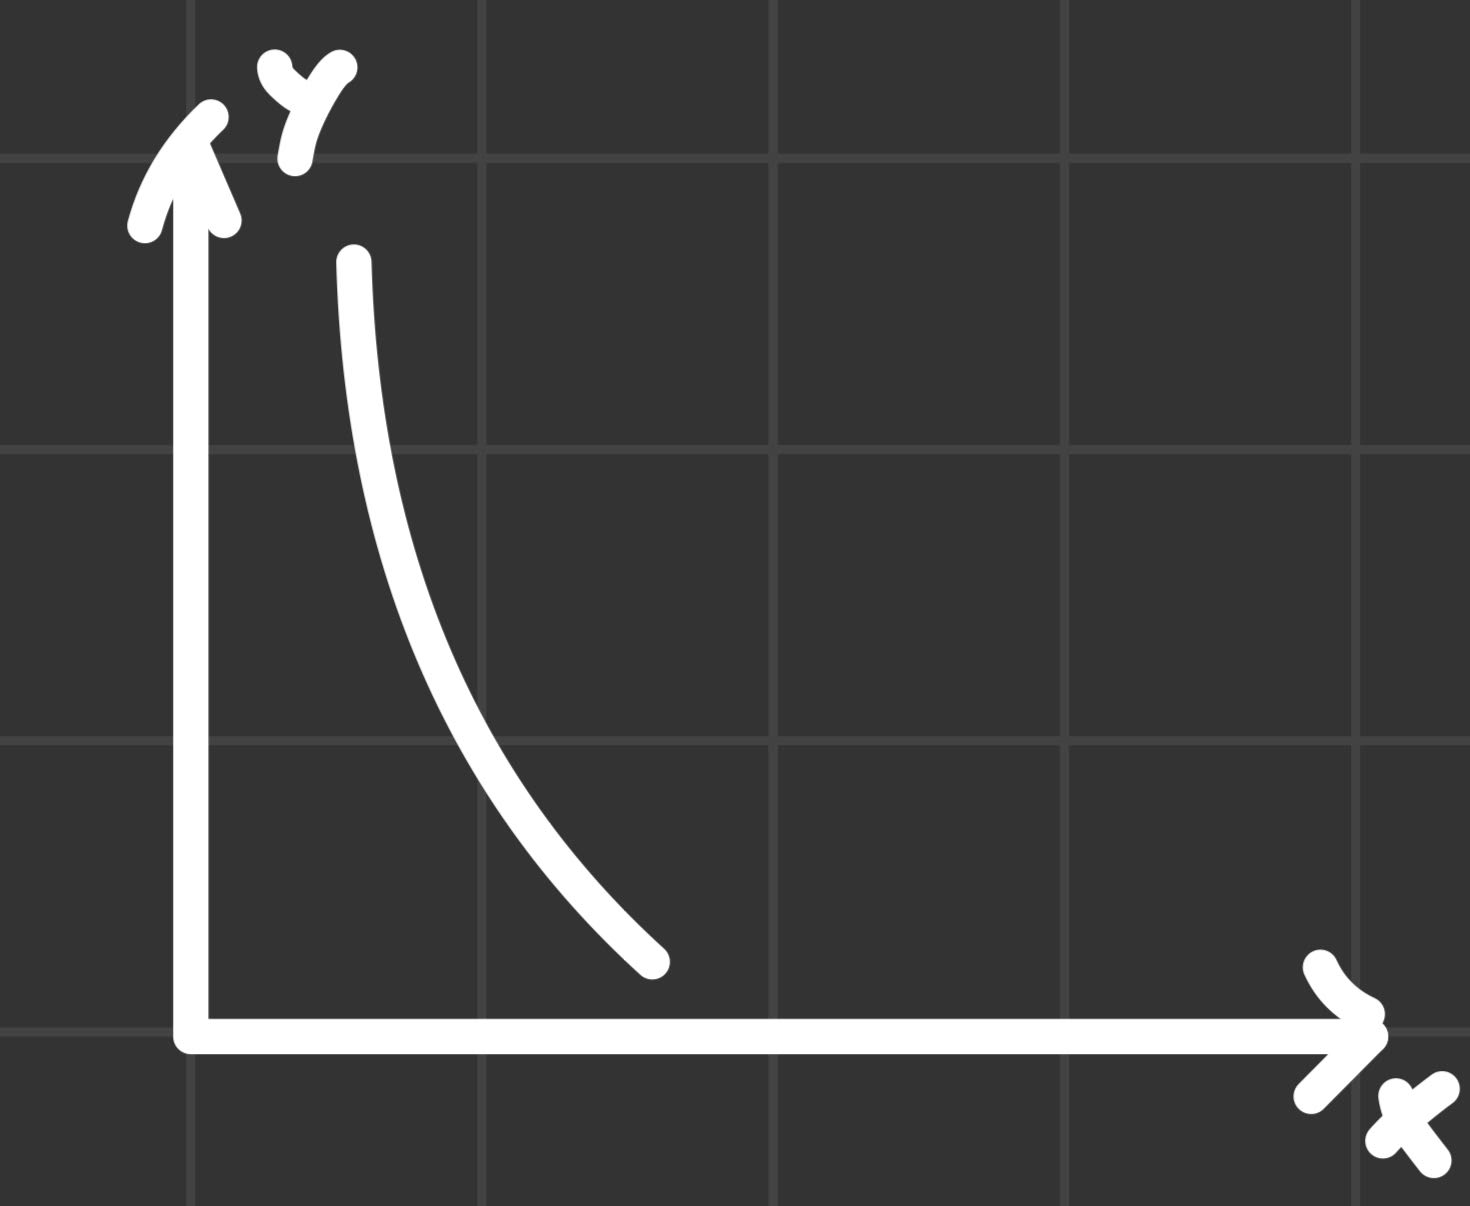
\includegraphics[width=0.25\linewidth]{Adiabatica.jpg}
    \label{fig:placeholder}
\end{figure}
\noindent
La rappresentazione è sempre un iperbole ma più pendente. Abbiamo 3 leggi di trasformazione:
\begin{align}
    & T_i(V_i)^{\gamma-1}=T_f(V_f)^{\gamma-1} \\
    & P_iV_i^\gamma = P_fV_f^\gamma \\
    & T_i(P_i)^{\frac{1-\gamma}{\gamma}} =T_f(P_f)^{\frac{1-\gamma}{\gamma}}
\end{align}
Il $\gamma$ che appare corrisponde a $\frac{c_P}{c_V}$. L'adiabatica capita spesso, questo perchè avendo tre leggi di trasformazione risulta complicato capire quale applicare.
\subsubsection{Politropica}
Fuori da 4 quattro trasformazioni individuiamo una quinta trasformazione detta politropica, con cui indichiamo una trasformazione generica. Nel caso in cui abbiamo questa trasformazione utilizziamo:
\subsection{Primo Principio della termodinamica}
\begin{equation}
    \Delta U=Q+W
\end{equation}
Dove $\Delta U$ corrisponde all'\textbf{energia interna del sistema termodinamico}, infatti per cambiare lo stato energetico del gas gli do calore e lavoro. Questa energia dipende dallo stato termodinamico del gase e quindi dallo stato delle molecole interne. Dobbiamo capire come legarlo alle tre variabili.
\subsubsection{Energia interna Isocora-Isobara-Adiabatica-Isoterma}
Siccome $Q=nc_V\Delta T$ e $W=0$ abbiamo che:
\begin{equation}
    \Delta U=Q+W \xrightarrow[]{} \Delta U=Q \xrightarrow[]{} \Delta U = nc_V\Delta T
\end{equation}
Risulta essere così per tutte le trasformazioni nell'adiabatica:
\begin{equation}
    \Delta U=Q+W \xrightarrow[]{} \Delta U=W \xrightarrow[]{} \Delta U = nc_V\Delta T
\end{equation}
Nell'isoterma invece:
\begin{equation}
    \Delta U =0
\end{equation}
Nella politropica:
\begin{equation}
    \Delta U = nc_V\Delta T \xrightarrow[]{} nc_V\Delta T = W+Q
\end{equation}
\subsection{Calori Specifici}
Apriamo una parentesi sui calori specifici, solitamente sono sempre dati basta leggere attentamente il testo. Infatti in un \textbf{adiabatica} $c=0$. L'altra differenziazione è data dal tipo di gas i quali hanno sempre gli stessi valori di $c_V \ e \ c_P$, i \textbf{monoatomici (gas nobili)} hanno: 
\begin{equation}
    c_V= \frac{3}{2}R \ \ \ \ c_P=\frac{5}{2}R \ \ \ \ \gamma=\frac{5}{3}=1.7 
\end{equation}
I \textbf{biatomici} invece:
\begin{equation}
    c_V= \frac{5}{2}R \ \ \ \ c_P=\frac{7}{2}R \ \ \ \ \gamma=\frac{7}{5}=1.4 
\end{equation}
\section{Lezione 12}
\subsection{Introduzione}
Questa lezione è dedicata principalmente agli esercizi, abbiamo svolto due esercizi del mazzoldi che introducono un pochino la metodologia utilizzata per risolvere gli esercizi, un terzo il quale ci introduce i cicli termodinamici e il rendimento.
\subsection{Come risolvere gli esercizi di termodinamica}
Analizzando i due esercizi capiamo come la risoluzione degli esercizi (almeno per adesso) dipenda strettamente dall'utilizzo delle equazioni e delle leggi di trasformazione. Infatti mettendo queste ultime a sistema riusciamo a trovare le incognite richieste. Quindi fondamentale avere chiara la trasformazione e la sua legge e convertire le unità di misura. Le \textbf{coordinate termodinamiche} indicano lo \textbf{stato termodinamico} e quindi richiedono di calcolare in quel punto \textbf{pressione, volume e temperatura}. Quindi quello che ho capito per adesso è che la cosa che conviene di più è scrivere le leggi di trasformazione delle trasformazioni che ho, lasciando per ultima la adiabatica in cui scegliamo la legge in base a quello che ci serve di più.
\subsection{Rendimento di un ciclo}
Con i cicli termodinamici si chiedono i \textbf{rendimenti}. I rendimenti sono una misura dell'efficienza termodinamica, la quale è stata introdotta dall'uomo. Ovvero vogliamo fare in modo che la maggior parte del calore venga assorbito e trasformato in lavoro. Per introdurre il rendimento consideriamo un ciclo termodinamico (un'insieme di trasformazioni) come un'unica trasformazione generale in cui lo stato iniziale è uguale allo stato finale. Consideriamo quindi la trasformazione politropica in cui sappiamo valere il \textbf{primo principio della termodinamica}:
\begin{equation}
    \Delta U = W+Q 
\end{equation}
Dato che la temperatura iniziale è uguale alla temperatura finale, $\Delta U = nc_V\Delta T\xrightarrow[\Delta T=0]{}\Delta U=0$. Avremo quindi dato che in questa trasformazione generale avvengono diversi passaggi di lavoro e di calore:
\begin{equation}
    0=W+Q \xrightarrow[]{} 0=\sum_i W_i+\sum_i Q_i \xrightarrow[]{} \sum_i W_i= \sum_i Q_i
\end{equation}
Questo possiamo scriverlo in questo modo dato che i lavori e i calori possono essere ceduti o assorbiti e avere quindi segno opposto. Infatti se il \textbf{calore o il lavoro} vengono assorbiti li consideriamo \textbf{positivi} se vengono ceduti li consideriamo \textbf{negativi}. Infatti vorrei che il gas assorba totalmente il calore per produrre più lavoro possibile e questo ha un costo in termini di risorse dato che per avere lavoro durante la trasformazione avrò anche calore ceduto. Vorremmo quindi più calore assorbito possibile con meno calore ceduto possibile. Introducendo il rendimento come:
\begin{equation}
    \eta = \frac{\sum_iW_i}{Q_A}=\frac{\sum_iQ_i}{Q_A}=\frac{Q_A-Q_C}{Q_A}=1-\frac{\sum_iQ_{Ci}}{\sum_iQ_{Ai}}
\end{equation}
Quindi inizialmente il rendimento è una misura che mi dice lavoro arrivato all'esterno su calore assorbito. Sappiamo che calore e lavoro possono scambiarsi e quindi in realtà mi interessa quanto è il calore che immetto (che successivamente si trasformerà in lavoro) su quanto calore assorbito ho. I calori immessi quindi diventeranno calori ceduti e calori assorbiti (nella frazione appaiono come dei termini, in realtà sarebbero sommatorie). Una nota importante è che \textbf{tutti i calori vanno messi positivi} e che i calori ceduti devono essere minori di quelli assorbiti, il \textbf{rendimento non può essere negativo $0<\eta<1$}. Un'altra osservazione è che il $\Delta T$ in termodinamica non è $T_{finale}-T_{iniziale}$ ma $T_{maggiore}-T_{minore}$.
\subsection{Esercizi d'esame}
Generalmente quello che ci aspettiamo negli esercizi d'esame è che i dati non sono assoluti e quindi per trovare il rendimento avremo probabilmente tutte le variabili in funzione delle altre. Generalmente i calori sono in \textbf{funzione di T} e raramente di V di conseguenza le temperature hanno la priorità nei calcoli. Solitamente i cicli vanno risolti scrivendo le leggi di trasformazione e iniziando i calcoli dalla trasformazione che più preferisco. 
\subsubsection{Calori assorbiti e Calori ceduti}
Per scrivere il rendimento ho bisogno di capire se i calori sono ceduti o assorbiti. Nell \textbf{isocora e isobara} se la temperatura aumenta stiamo \textbf{assorbendo calore} se diminuisce stiamo \textbf{cedendo calore}. Nell'\textbf{adiabatica} il calore è 0 quindi non ci si può sbagliare. Nell'\textbf{isoterma} invece, se il calore è negativo allora sto \textbf{cedendo calore} positivo viceversa, si può fare un ragionamento anche in termini di lavoro se è $W>0$ allora sto \textbf{assorbendo calore} il contrario viceversa.
\section{Lezione 13}
\subsection{Risoluzione esercizi d'esame}
Anche questa lezione è completamente dedicata agli esercizi di termodinamica, in particolare al calcolo del rendimento. Infatti approfondiamo un pochino i ragionamenti fatti prima e capiamo che la cosa più conveniente da fare per risolvere gli esercizi d'esame è \textbf{scrivere la formula del rendimento, capire i calori ceduti e assorbiti, scriverli formalmente e da lì trovare quelle incognite con le leggi di trasformazione}. Generalmente si troveranno volumi e temperature noi daremo la \textbf{priorità alle temperature}, infatti vorremmo scrivere tutto in funzione di una temperatura in modo tale da semplificarla. Generalmente in tutti gli esercizi semplificheremo anche n e R. 
\subsubsection{Calori assorbiti e Calori ceduti}
Per quanto riguarda i calori, considerando che le temperature non sono quasi mai date bisogna trovare un'altra metodologia e questo possiamo farlo guardando semplicemente il grafico e i volumi. Infatti se abbiamo un \textbf{aumento dei volumi allora il calore sarà assorbito}. Se abbiamo lo stesso volume, basterà vedere chi si trova più in alto nel grafico e quindi chi ha più pressione.
\subsubsection{Metodologie per gli esercizi}
Tornando agli esercizi, abbiamo detto che vogliamo scrivere tutto in funzione di una temperatura, che generalmente è $T_a$, per fare questo con le leggi di trasformazione, devo trovare tutte le temperature in funzione di $T_a$. Nel rendimento solitamente possiamo trovare anche i volumi e anche in questo caso vorremmo scrivere tutto in funzione di uno solo. Quindi riepilogando, scrivo il rendimento, trovo tutte le temperature in funzione di una sola (con i dati del testo o con le leggi di trasformazione) se ci sono volumi li scrivo in funzione di uno solo e cerco di semplificare. Importante negli esercizi nonostante non ho variabili assolute, il \textbf{rendimento è assoluto (è un valore)}. Vediamo poi un'altro esercizio, che cambia leggermente, infatti abbiamo una trasformazione detta \textbf{espansione lineare} che sarebbe una politropica per cui il calore, può esser trovato con il primo principio della termodinamica:
\begin{equation}
    \Delta U = Q + L
\end{equation}
Va fatta in realtà una precisazione sul segno del lavoro, infatti il \textbf{lavoro va preso positivo se il gas viene compresso (minor volume) negativo se viene espanso}. Quindi esempio se ho una trasformazione $D\xrightarrow[]{}A$ $V_A>V_D$ allora $\Delta U = Q - L$ se ho $V_D>V_A$ allora $\Delta U = Q + L$.
\subsubsection{Lavoro nel rendimento}
In caso appaia il lavoro nel rendimento, bisogna ricordarsi che il lavoro è uguale all'area sottesa alla singola trasformazione. Infatti in quest esempio:
\begin{figure}[H]
    \centering
    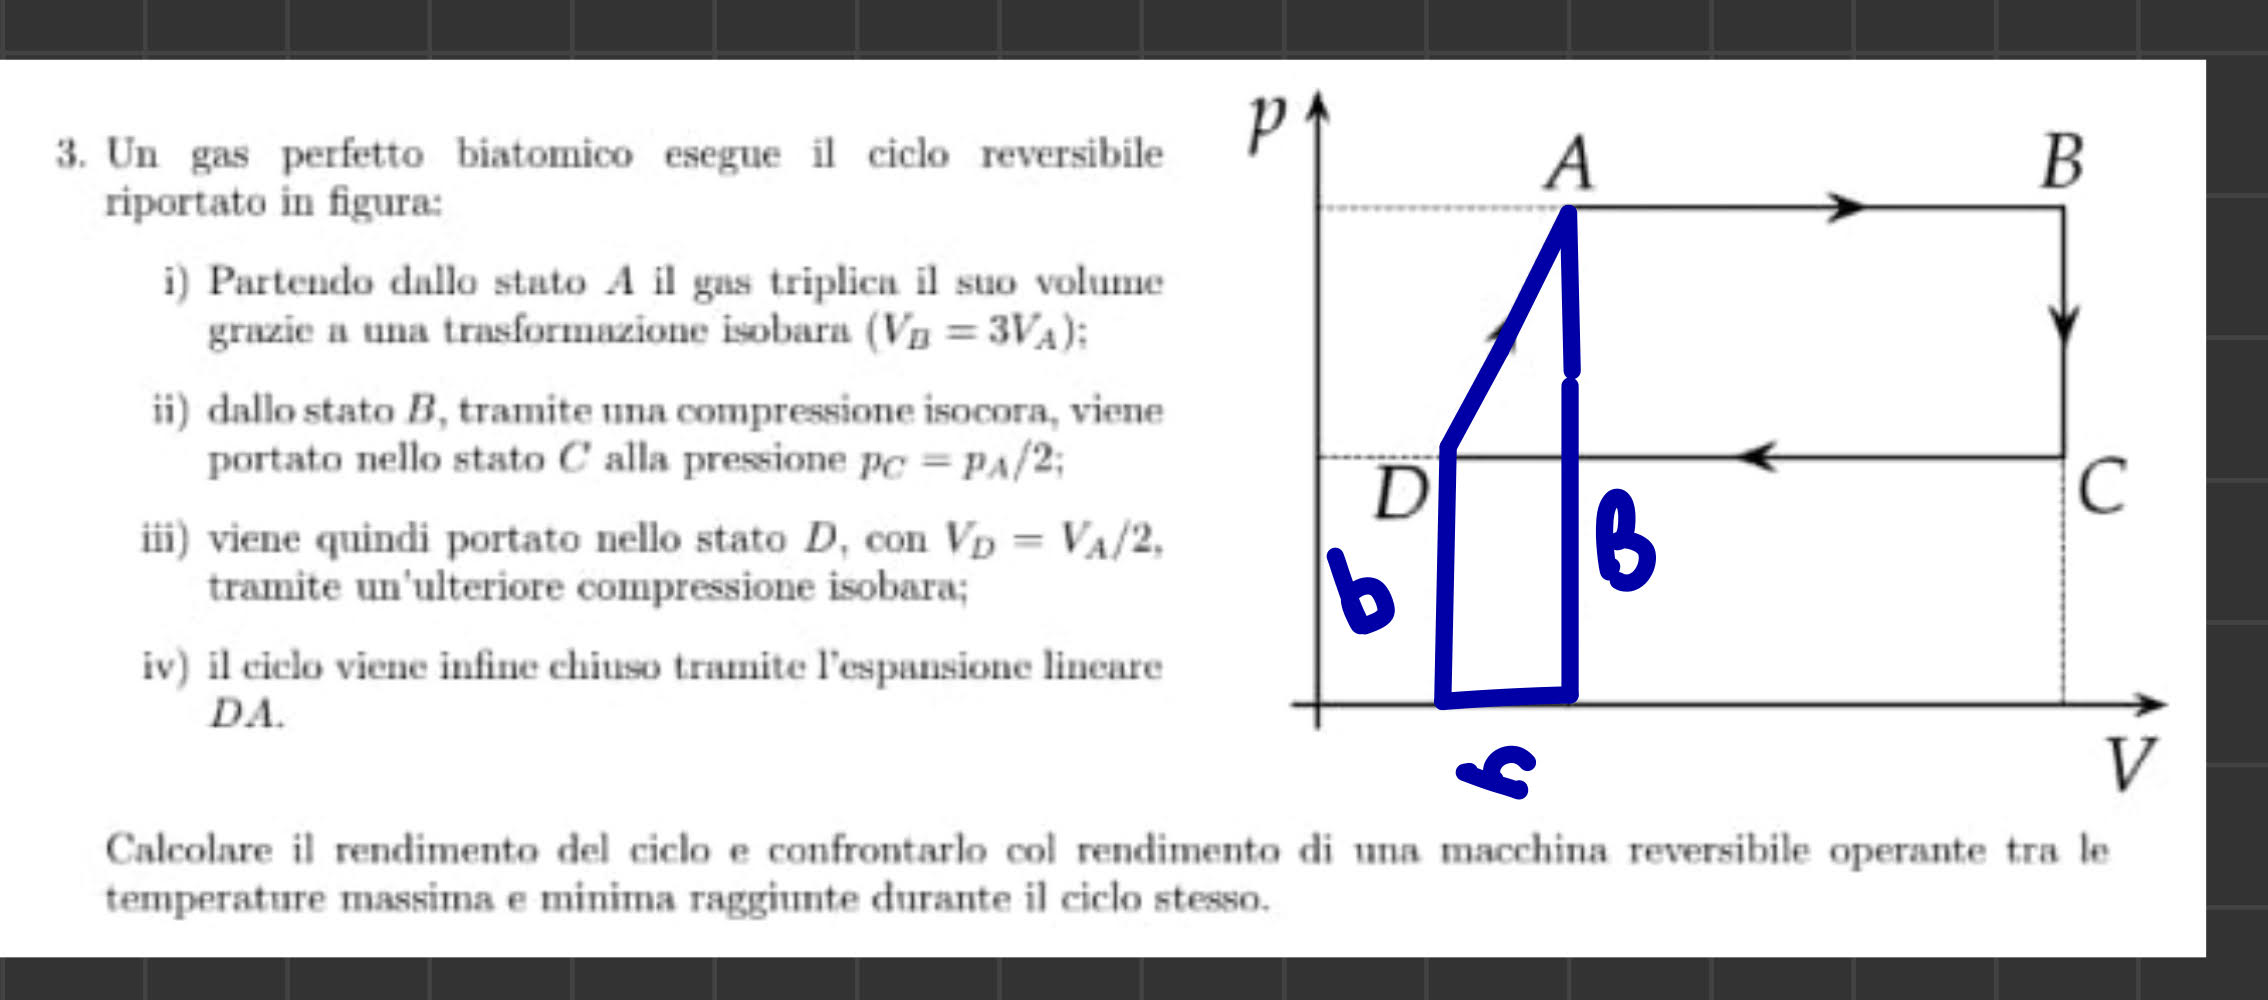
\includegraphics[width=0.7\linewidth]{LavoroERendimento.jpg}
    \label{fig:placeholder}
\end{figure}
Il lavoro sarà uguale all'area del trapezio in blu, e quindi:
\begin{equation}
    L = \frac{(b+B)*h}{2}= \frac{(P_D+P_A)*(V_A-V_D)}{2}
\end{equation}
Ultima osservazione, la differenza di temperatura del $\Delta U$ è sempre $T_{finale}-T_{iniziale}$.
\section{Lezione 14}
\subsection{Introduzione}
Questa lezione, è incentrata principalmente sulla nuova tipologia di esercizi di termodinamica, quelli che riguardano una singola trasformazione.
\subsection{Problema del recipiente adiabatico}
Questi problemi, sono problemi che si affrontano più con il ragionamento che praticamente. Infatti bisogna prima capire, \textbf{di che trasformazione stiamo parlando}, per farlo leggo il testo e inizio a escludere le trasformazioni che non possono essere.
\begin{figure}[H]
    \centering
    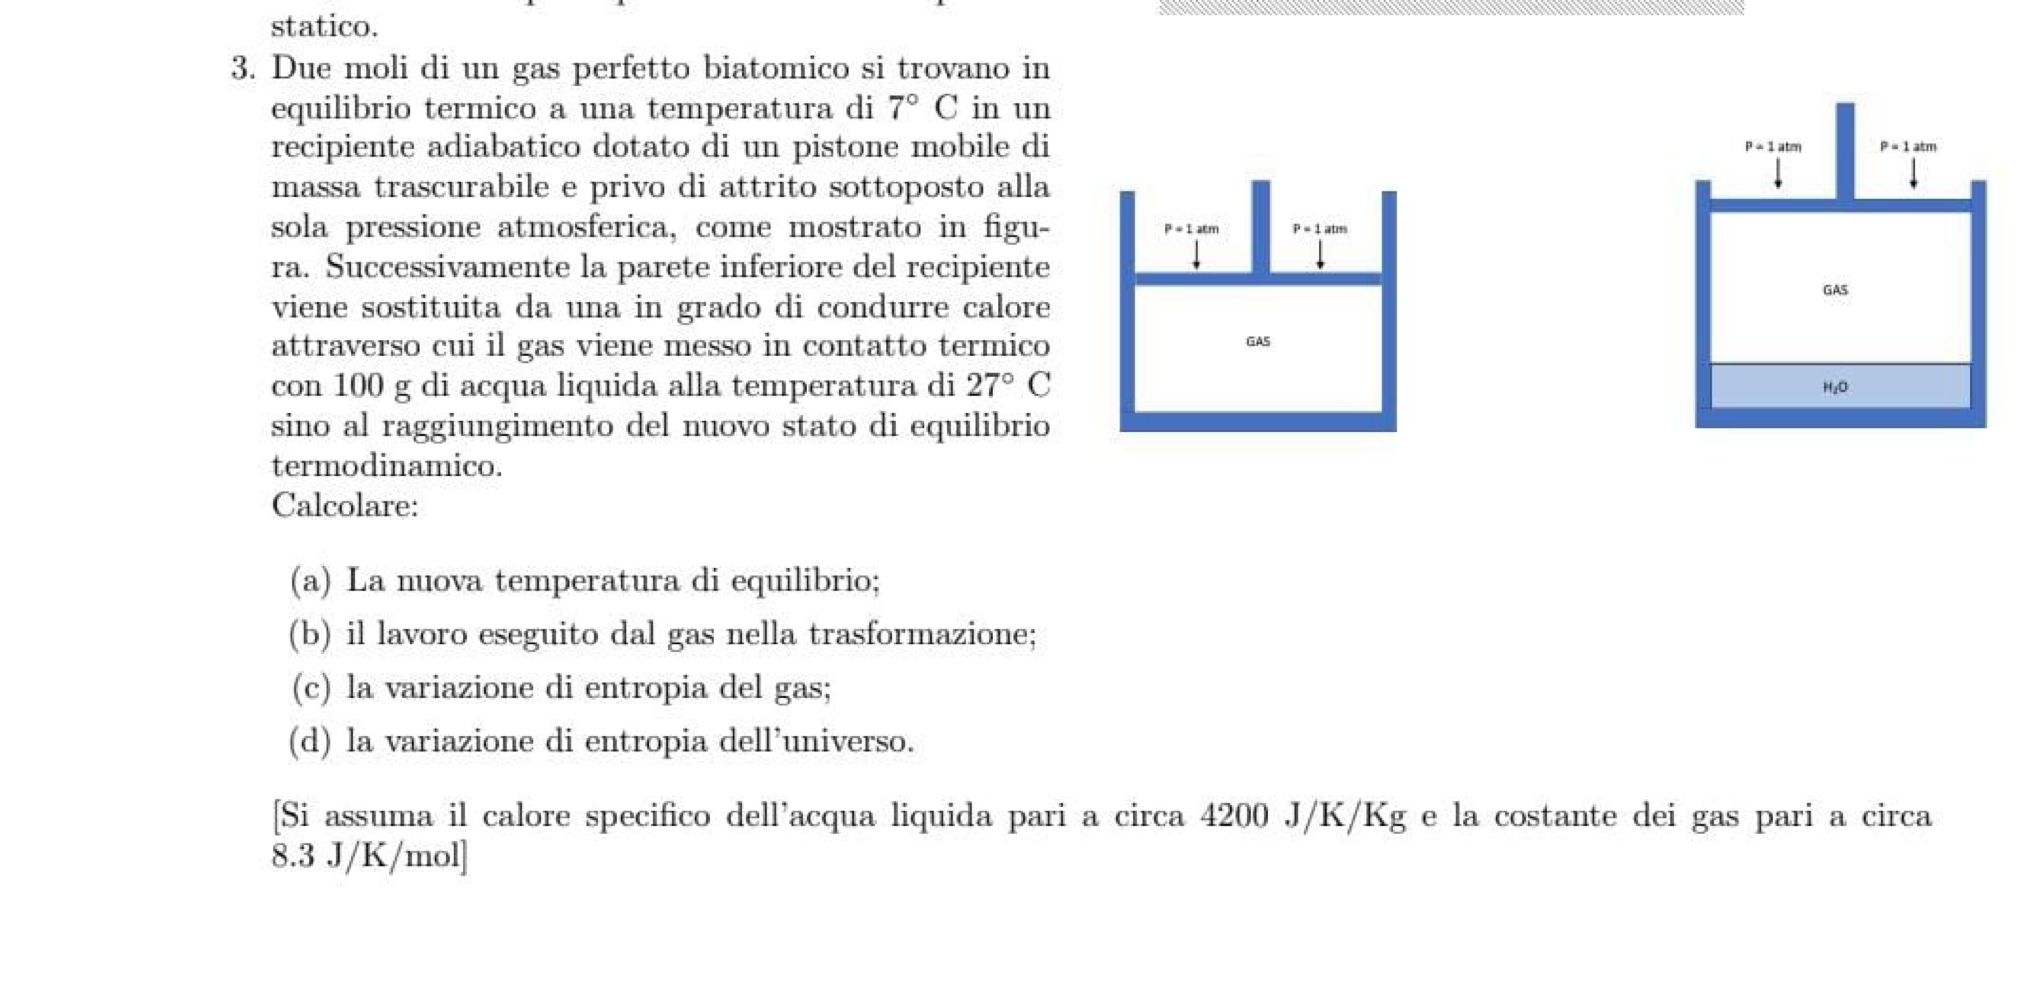
\includegraphics[width=0.9\linewidth]{ProblemaDelRecipienteAdiabatico.jpeg}
    \label{fig:placeholder}
\end{figure}
\noindent
Essendoci due corpi aventi temperatura differente, sappiamo che vi sarà uno scambio di temperatura e di conseguenza riusciamo a escludere l'isoterma. Il gas riceverà calore dall'acqua e di conseguenza si espanderà, per questo motivo escludiamo l'isocora. Per quanto riguarda l'\textbf{isobara}, consideriamo un'adattamento quasi istantaneo tra la pressione interna e la pressione esterna, di conseguenza la pressione esterna non cambia e avremo quindi che il gas si sta espandendo alla pressione isobara di un'atmosfera. Quindi quello che abbiamo capito adesso è che il gas effettua una trasformazione \textbf{isobara} ma se consideriamo anche il recipiente adiabatico questo fa si che il gas abbia una trasformazione sia adiabatica che isobara. Giungiamo alla conclusione che la trasformazione considerata è \textbf{politropica} e quindi vale solamente il primo principio della termodinamica. Però avevamo capito che il gas aveva una trasformazione che ammetteva il cambio di temperatura, arriviamo quindi a una contraddizione. In questi esercizi andremo a considerare tutto il sistema e per questo motivo dovremo capire anche l'acqua che tipo di trasformazione effettua. Ovviamente per l'acqua la trasformazione è \textbf{isocora}. Scriviamo il primo principio della termodinamica:
\begin{equation}
    \Delta U = Q+L
\end{equation}
Dato che il gas viene espanso, il segno del lavoro è negativo. Inoltre c'è da fare un'altro ragionamento, acqua e gas seguono due trasformazioni differenti per questo motivo le variazioni di energia interna del sistema devono considerare sia l'acqua che il gas. Apriamo quindi una parentesi specificando che la \textbf{variazione di energia interna in un solido o in un liquido} è uguale a:
\begin{equation}
    \Delta U = mc\Delta T
\end{equation}
dove m è la massa e c è il calore specifico che solitamente è dato nel testo. Allora riscriviamo il primo principio della termodinamica:
\begin{equation}
    \Delta U_{gas} + \Delta U_{acqua} = -L \ \  \xrightarrow{} \ \ nc_V\Delta T + mc\Delta T=-L
\end{equation}
Dobbiamo aprire un'altra parentesi per quanto riguarda il lavoro, in questo caso guardando la situazione fisica, capiamo che \textbf{l'unico a scambiare lavoro con l'esterno, è il gas, il quale sta compiendo una trasformazione isobara}, motivo per il quale andremo a scrivere semplicemente il suo di lavoro.
\begin{equation}
    nc_V\Delta T + mc\Delta T=-P* \Delta V
\end{equation}
Esplicitando le temperature e i volumi capiamo quali sono le vere incognite, infatti le temperature iniziali già le abbiamo, le finali ovviamente coincidono, avendo pressione del gas e temperatura iniziale del gas troviamo facilmente con l'equazione dei gas perfetti il volume iniziale del gas. Inoltre ricordo che quest'equazione è nostro obiettivo scriverla in funzione di una sola temperatura, quella finale, in modo tale da poterla trovare successivamente, infatti vado a esprimere il volume finale in funzione della temperatura finale grazie alla legge di trasformazione dell'isobara compiuta dal gas. Di lì riesco a trovare lavoro e temperatura finale.
\subsection{Entropia}
Iniziamo a parlare di entropia, la quale è una misura che dipende dalle variabili di stato ed è una \textbf{misura dello stato di disordine della materia}. Infatti ad esempio, aumentando la temperatura, le particelle iniziano a muoversi più velocemente e di conseguenza aumenta anche l'entropia
\subsubsection{Entropia Latente}
Parliamo anche di entropia latente che \textbf{misura il disordine tra i cambiamenti di stato}. Infatti volendo fare un esempio, prendiamo la trasformazione da ghiaccio a liquido dell'acqua, quello che succede è che il calore è occupato a sciogliere i legami facendo muovere le particelle più velocemente e per questo motivo non ho aumento di temperatura ma ho ovviamente un'aumento di entropia. Ogni trasformazione ha un'entropia differente:
\begin{align}
    & \Delta S = nRln(\frac{V_F}{V_I}) \ \ \ \ o \ \ \ \ \Delta S=\frac{Q}{T} \ \ \ \ Isoterma \\
    & \Delta S = nc_Pln(\frac{T_F}{T_I}) \ \ \ \ Isobara \\
    & \Delta S = nc_Vln(\frac{T_F}{T_I}) \ \ \ \ Isocora \\
    & \Delta S = 0 \ \ \ \ Adiabatica 
\end{align}
Specifichiamo inoltre: $\Delta S>0$ allora si sta assorbendo calore, $\Delta S <0$ si sta cedendo calore.
\subsubsection{Variazione dell'entropia dell'universo}
Un'altra richiesta tipica di questo tipo di problema, è la variazione di entropia dell'universo. Dobbiamo considerare quindi il recipiente e l'ambiente. In questo caso l'ambiente fa una trasformazione adiabatica ($Q=0 \ \ \Delta S = 0)$, infatti non vi è alcun passaggio di calore tra interno e esterno. Generalmente è sempre così a eccezione di quando siamo in presenza di \textbf{sorgenti}. Consideriamo una sorgente, tutto ciò che assorbe o cede calore tra interno e esterno, quest'ultima può essere \textbf{limitata} o \textbf{illimitata}. Se la sorgente è illimitata, consideriamo una trasformazione \textbf{isoterma}, infatti il gas all'esterno è illimitato e per questo motivo posso dargli tutto il calore che voglio ma non cambierà temperatura. Se la sorgente è limitata il discorso cambia, il testo dirà "c'è una sorgente a una determinata temperatura". Si fa ipotesi comunque di una trasformazione \textbf{isoterma} e quindi la temperatura non cambia. Se invece parla di una sorgente tipo "due cubetti di ghiaccio" per trovare la temperatura di equilibrio si fa un ragionamento analogo a questo esercizio. Se ho una sorgente che scambia calore con l'esterno, ho una temperatura di equilibrio quando il calore cessa di esserci e so quindi che $T_{F, Sorgente}=T_{F, ambiente}$. Inoltre dato che la variazione di entropia dipende da inizio e fine lungo un ciclo avremo $\Delta S=0$. Anche in caso di trasformazioni irreversibili. Finita questa parentesi ricordiamo il calcolo come:
\begin{equation}
    \Delta S_{Recipiente}+\Delta S_{Ambiente}= \Delta S_{Gas}+\Delta S_{acqua} 
\end{equation}
L'ambiente fa una trasformazione adiabatica.
\subsection{Trasformazioni Irreversibili}
Negli esercizi, possiamo trovarci in una situazione in cui una trasformazione è irreversibile e quindi dallo stato finale non posso tornare a quello iniziale, può essere di qualsiasi tipo e \textbf{non posso applicare la sua legge di trasformazione}. Nonostante non possa applicare le leggi di trasformazione nel caso in cui siamo in presenza di una trasformazione in cui si mantiene costante qualcosa, quello può andare da inizio a fine e da fine a inizio. Oltre a queste accortezze gli esercizi si risolvono in maniera analoga.
\subsection{Lavoro in una politropica}
\begin{figure}[H]
    \centering
    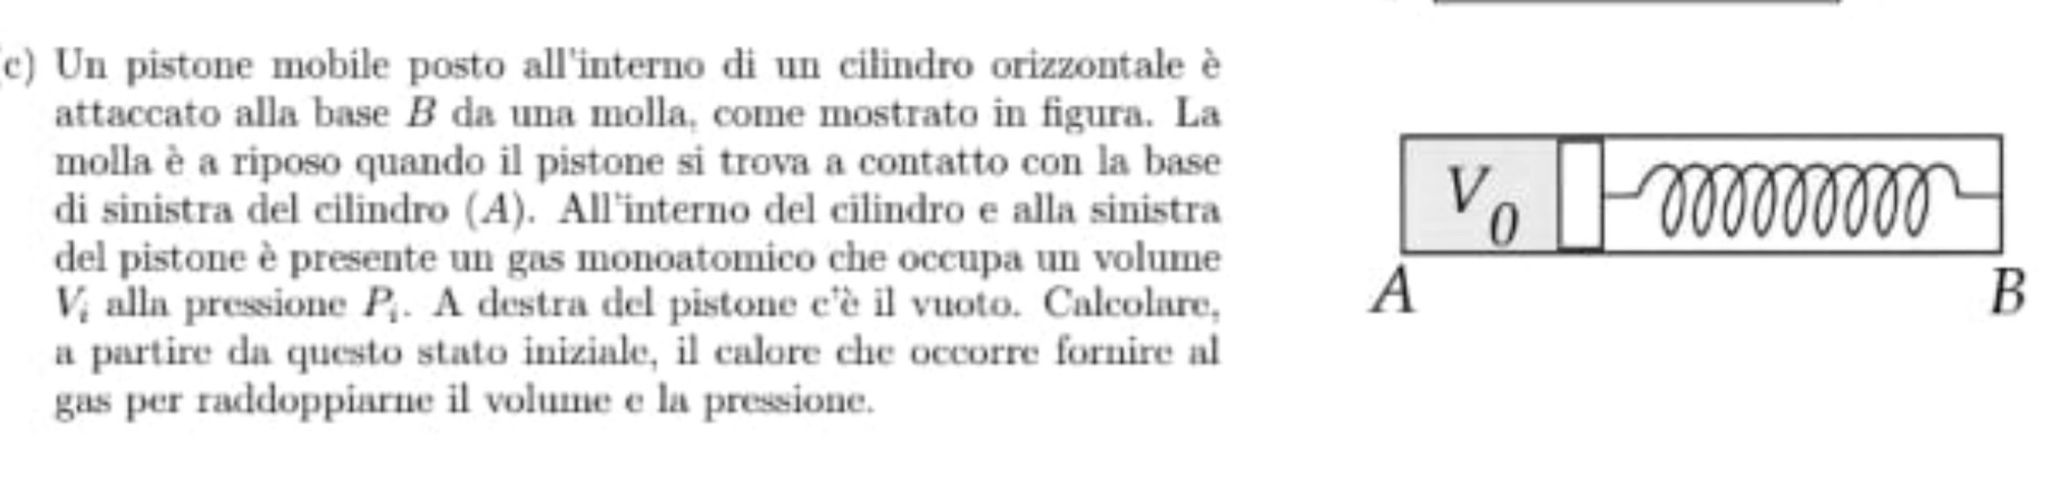
\includegraphics[width=0.8\linewidth]{LavoroInUnaPolitropica.jpeg}
    \label{fig:placeholder}
\end{figure}
Iniziamo ragionando come abbiamo precedentemente imparato, siccome la consegna parla di passaggio di calore, siamo sicuri che non siamo in presenza di un adiabatica, inoltre parla di raddoppio di volume e pressione, il che esclude anche la presenza di rispettivamente un isocora e un isobara, ci resta da determinare se la trasformazione è isoterma, e questo possiamo capirlo anche utilizzando l'equazione dei gas perfetti, è chiaro che se calcoliamo la temperatura con i volumi e le pressioni iniziali questa differirà rispetto a quella calcolata con entrambi raddoppiati. Siamo quindi in presenza di una politropica per cui vale l'unica legge, il primo principio della termodinamica:
\begin{equation}
    \Delta U = Q - L \ \ \ \ \xrightarrow[]{} Q = \Delta U + L
\end{equation}
Qui arriviamo a un problema, $\Delta U$ lo sappiamo calcolare, il lavoro invece no. Se andiamo a raffigurare sul piano di clapeyron la situazione e ci ricordiamo che il lavoro è l'area sottesa alla trasformazione troviamo questo:
\begin{figure}[H]
    \centering
    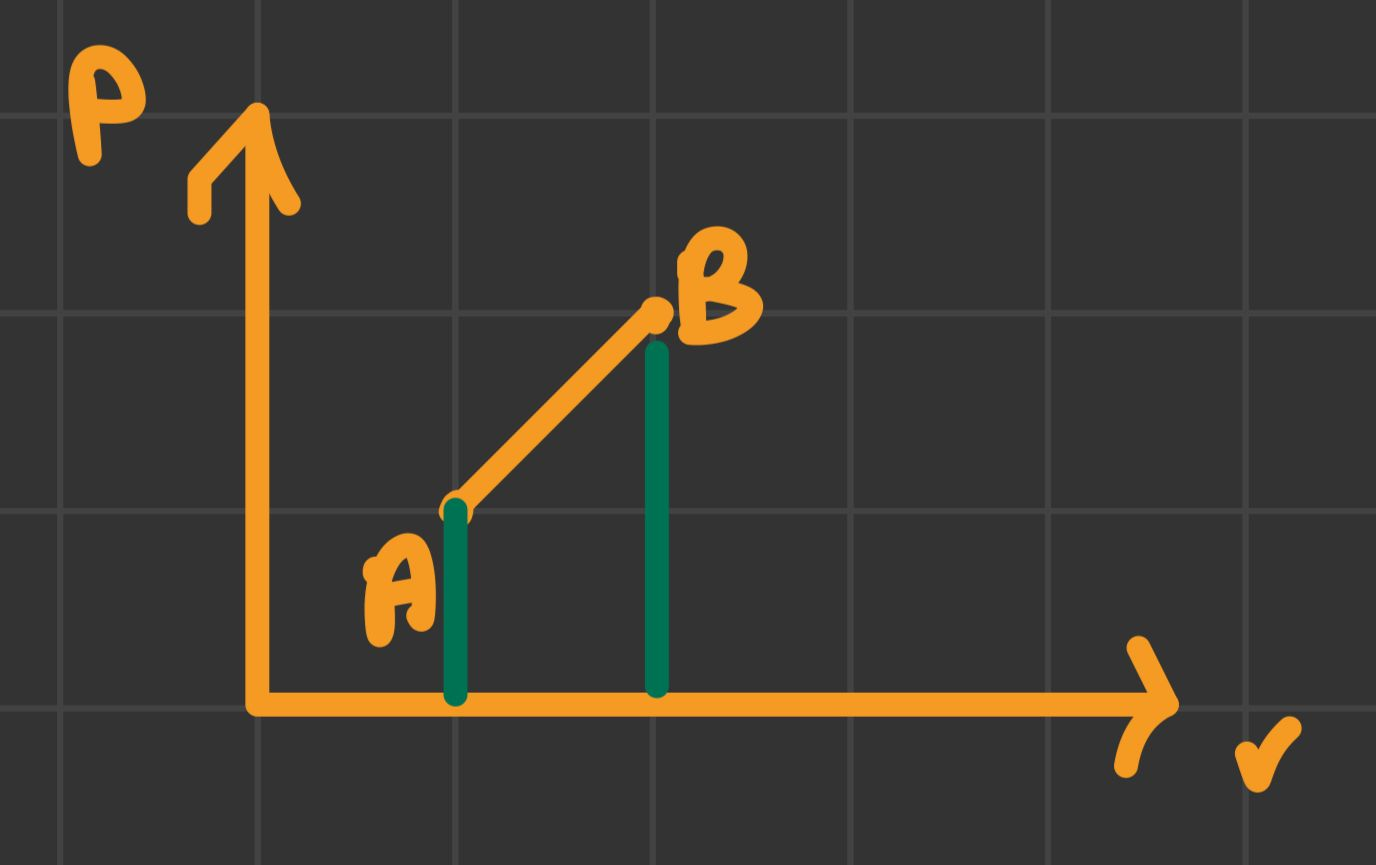
\includegraphics[width=0.3\linewidth]{LavoroDiUnaPolitropica.jpeg}
    \label{fig:placeholder}
\end{figure}
\noindent
e quindi troviamo facilmente il lavoro come l'area del trapezio. Nota: il risultato di questo problema non sarà assoluto.
\newpage
\section{Lezione 15}
\subsection{Introduzione}
In questa lezione andiamo a finire tutte le cose che ci erano rimaste, in particolare le ultime richieste dei problemi di termodinamica e le oscillazioni del pendolo semplice e composto.
\subsection{Esercizio 19 giugno 2025}
\begin{figure}[H]
    \centering
    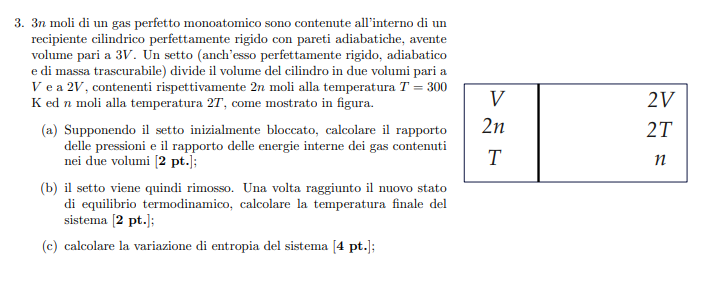
\includegraphics[width=0.8\linewidth]{EsercizioTermodinamicaConSetti.PNG}
    \label{fig:placeholder}
\end{figure}
\noindent
Cerchiamo di capire quello che sta succedendo per poter ragionare sulla prima richiesta del problema. Quando il setto è bloccato consideriamo il gas in due parti separate, la prima parte conterrà il gas a, la seconda il gas b. Ragionando con l'equazione di stato dei gas perfetti, capiamo facilmente come calcolare i rapporti, infatti calcolando le pressioni e facendone il rapporto, i dati parametrici si semplificano, trovando un valore assoluto. Stessa cosa succede per le energie interne, qui c'è bisogno di fare una precisazione, il problema richiede le energie interne e non la variazione di energia interna, \textbf{motivo per il quale andremo a utilizzare invece di $\Delta T$ solamente $T_A \ \ e \ \ T_B$}. Anche questo rapporto viene assoluto. La richiesta b è quella che ci da lo spunto per parlare di qualcosa di nuovo, infatti come gli altri problemi cerchiamo di capire che trasformazione sta vivendo l'intero sistema. Il recipiente ha delle pareti adiabatiche, il che presuppone che non scambi calore con l'esterno di conseguenza, possiamo già dire che effettua una trasformazione \textbf{adiabatica}. Inoltre possiamo anche osservare che il volume complessivo del sistema non cambia e quindi effettua anche una trasformazione \textbf{isocora}. Per quanto riguarda le rimanenti, il problema non parla di pressioni e quindi non consideriamo una trasformazione isobara. All'interno vi è un cambio di temperatura e come dice anche il testo "calcolare la temperatura finale" il che vuol dire che la temperatura rimane costante e quindi escludo l'isoterma. Parliamo allora di una \textbf{politropica}, per cui sappiamo valere il primo principio della termodinamica. 
\begin{equation}
    \Delta U = Q + L
\end{equation}
Dato che il sistema effettua una trasformazione adiabatica $Q=0$, effettua anche una trasformazione isocora e quindi $L=0$. Di conseguenza avremo:
\begin{equation}
    \Delta U_A + \Delta U _ B=0
\end{equation}
Questo in realtà già c'è lo aspettavamo, si chiama \textbf{processo di diffusione libera} in cui i due gas si scambiano e $\Delta U = 0$. Da quest'equazione riesco facilmente a trovare la temperatura finale avendo tutti i dati di cui ho bisogno.
\begin{equation}
    nc_V(T_F-T_A)+nc_V(T_F-T_B)
\end{equation}
\subsubsection{Variazione di entropia di una Politropica}
Vediamo ora il punto c in cui ci chiede di calcolare la variazione di entropia del sistema. Ovvero la variazione di entropia del gas a e del gas b. In questo caso conviene ragionare sull'intero sistema. 
\begin{equation}
    \Delta S = \Delta S_A+\Delta S_B
\end{equation}
A tal proposito introduco il calcolo della variazione di entropia per quanto riguarda una politropica.
\begin{align}
    & \Delta S = nc_Vln(\frac{T_F}{T_I})+nRln(\frac{V_F}{V_I}) \\
    & \Delta S = nc_Vln(\frac{P_F}{P_I})+nc_Pln(\frac{V_F}{V_I}) \\
    & \Delta S = nc_Pln(\frac{T_F}{T_I})-nRln(\frac{P_F}{P_I})
\end{align}
Utilizzo la prima e trovo facilmente tutto quello che mi serve dato che il parametro sui volumi si semplifica. Ovviamente il risultato sarà parametrico rispetto a n. 
\subsection{Ultima tipologia esercizi termodinamica}
Vediamo ora l'ultima tipologia di esercizi di termodinamica:
\begin{figure}[H]
    \centering
    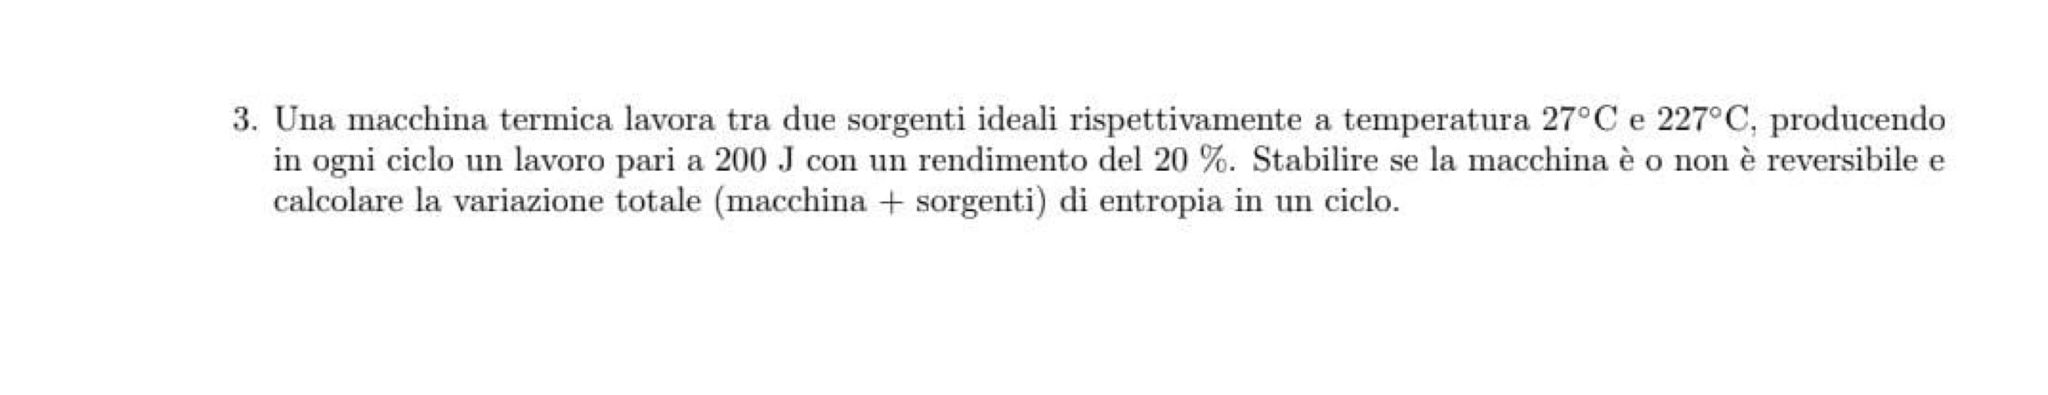
\includegraphics[width=0.9\linewidth]{UltimaTipologiaTermodinamica.jpeg}
    \label{fig:placeholder}
\end{figure}
\noindent
Per fare questo tipo di esercizi, ragioniamo la macchina termica come una blackbox ovvero sappiamo che equivale a un ciclo di trasformazioni ma non sappiamo quale. 
\subsubsection{Rendimento di Carnot}
Per risolvere questi esercizi, dobbiamo capire se la macchina è reversibile, per farlo dobbiamo calcolare il \textbf{rendimento della macchina di Carnot}. La macchina di Carnot anche detta ciclo di Carnot, è composta da \textbf{2 isoterme e 2 adiabatiche}, motivo per il quale troviamo il suo rendimento come:
\begin{equation}
    \eta = 1- \frac{T_{MIN}}{T_{MAX}}
\end{equation}
In questo caso giungiamo a un'approssimazione e utilizziamo proprio le temperature che ci da il testo. Per capire quindi se la macchina è reversibile dobbiamo avere:
\begin{equation}
    \eta = \eta_C
\end{equation}
In questo caso il rendimento è noto, è minore del rendimento di Carnot e quindi stabiliamo che il ciclo non è reversibile. 
\subsubsection{Entropia e sorgenti}
Noto questo, il problema ci chiede di calcolare la variazione totale di entropia in un ciclo. Per farlo dobbiamo ripetere i ragionamenti che avevamo fatto per entropia e sorgenti. Di fatti avremo:
\begin{equation}
    \Delta S_{Totale}=\Delta S_{Macchina} + \Delta S_{Sorgenti}
\end{equation}
Abbiamo detto che ragioniamo la macchina come un ciclo e quindi $\Delta S = 0$. Per quanto riguarda le sorgenti invece dobbiamo considerare la loro capacità termica e capire se questa è finita o infinita:
\begin{equation}
    C=\frac{m}{c}
\end{equation}
\begin{itemize}
    \item Se la capacità termica è \textbf{infinita} ovvero la sorgente scambia calore con il gas senza cambiare temperatura approssimiamo a una trasformazione isoterma in cui $\Delta S = \frac{Q}{T}$, non possiamo applicare l'altra considerando che non ho il volume di qualcosa di infinito. Ad esempio l'ambiente può esser composto d'aria, dandogli calore, l'aria non cambierà temperatura e quindi consideriamo la trasformazione \textbf{isoterma}. In questo caso la temperatura finale del gas tenderà sempre di più alla temperatura della sorgente.
    \item Se la capacità termica è \textbf{finita} dovrei trovare la temperatura di equilibrio tra la sorgente e il gas.
    \item Inoltre c'è da specificare che se il testo non mi da la possibilità di calcolare la capacità termica assumiamo la sorgente come \textbf{infinita}.
\end{itemize}
In questo caso assumiamo le capacità termiche infinite e calcoliamo:
\begin{equation}
    \Delta S_1 + \Delta S_2 = \frac{Q_1}{T_1}+\frac{Q_2}{T_2}
\end{equation}
Devo quindi calcolare questi calori, per farlo mi ricordo che il rendimento:
\begin{equation}
    \eta = 1- \frac{Q_C}{Q_A} = 0.2
\end{equation}
e che la variazione di lavoro per definizione:
\begin{equation}
    \Delta L = Q_A - Q_C = 200
\end{equation}
Metto a sistema e trovo i calori assorbiti e ceduti ma da parte del gas. Ho quindi bisogno di collegare quest'informazione alle sorgenti.
\begin{figure}[H]
    \centering
    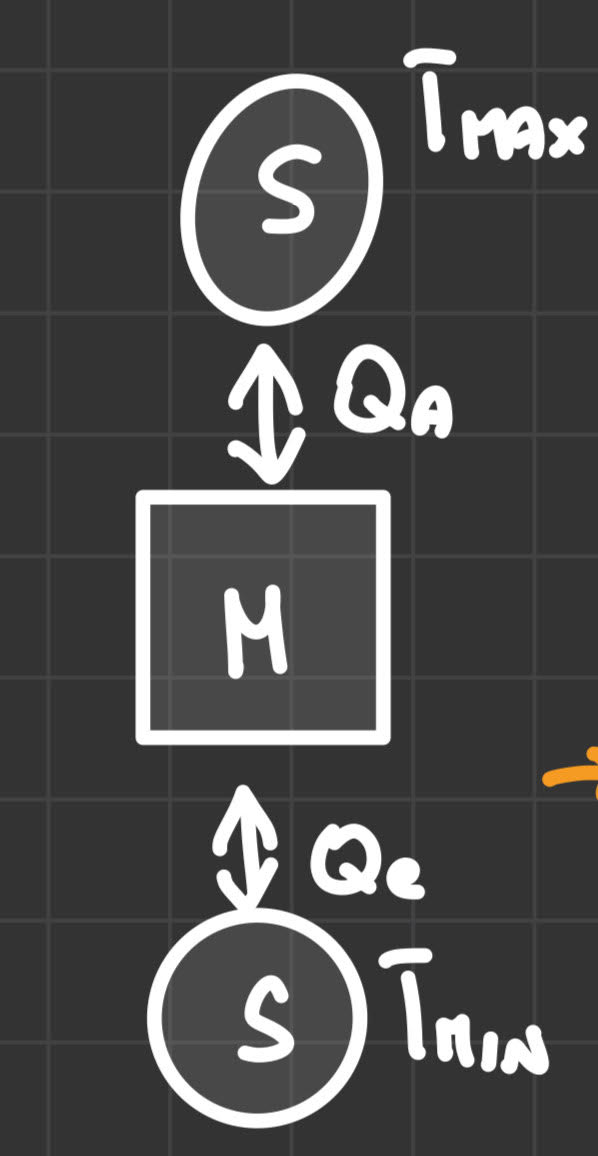
\includegraphics[width=0.2\linewidth]{ScambioDiCaloreTraSorgenti.jpg}
    \label{fig:placeholder}
\end{figure}
\noindent
Come si vede la sorgente con temperatura più alta sta cedendo calore, il quale appare come assorbito dalla macchina termica, mentre la sorgente con temperatura più bassa sta assorbendo calore e quindi appare come ceduto dalla macchina termica. In questo caso i calori non li prendiamo positivi dato che l'entropia può avere un valore negativo e quindi dato che la sorgente con temperatura maggiore si sta raffreddando assumiamo il suo calore come negativo:
\begin{equation}
    \Delta S = \frac{-Q_A}{T_1} + \frac{Q_C}{T_2}
\end{equation}
\newpage
\subsection{Centro di massa di un sistema di corpi rigidi}
\begin{figure}[H]
    \centering
    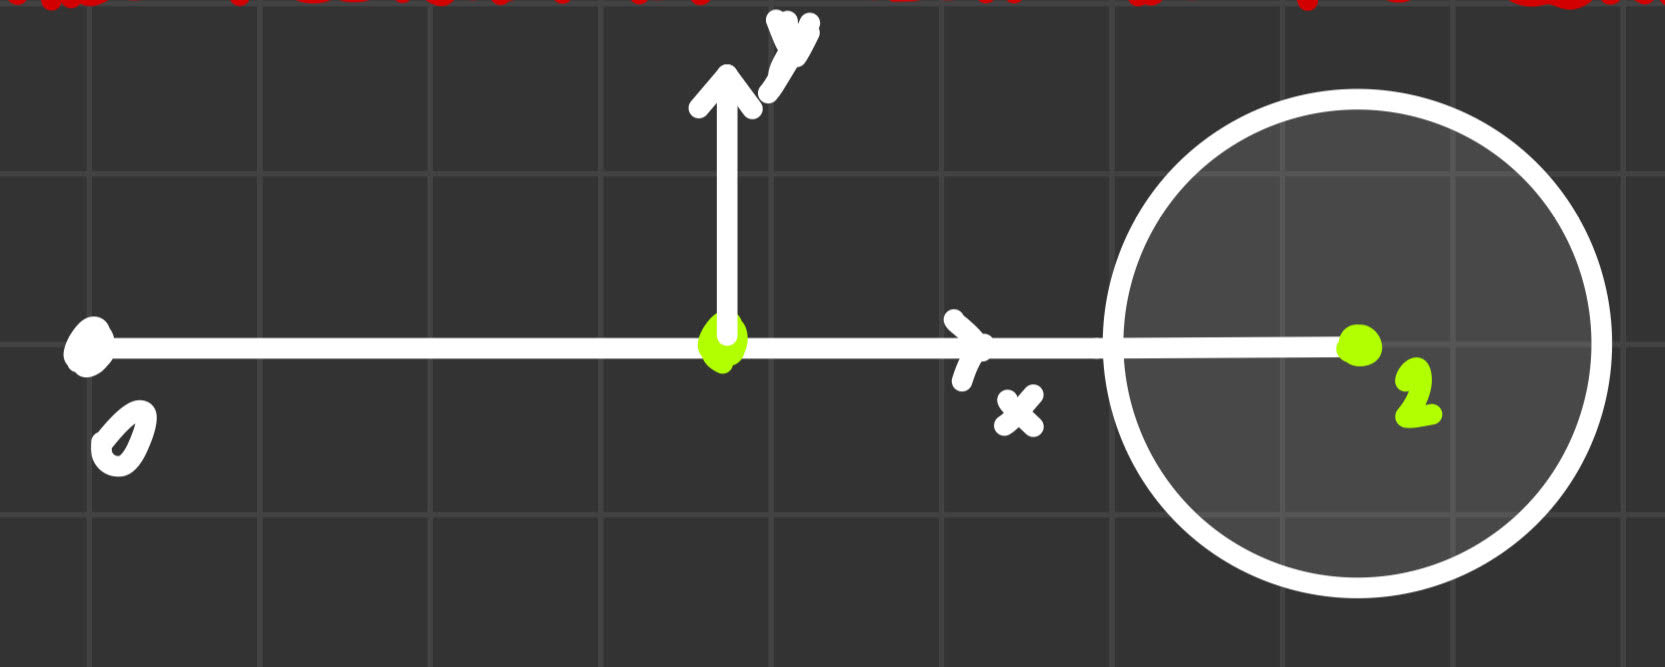
\includegraphics[width=0.5\linewidth]{CentroDiMassaDiPiùCorpiRigidi.jpg}
    \label{fig:placeholder}
\end{figure}
\noindent
Vediamo ora una delle cose che ci erano rimaste da fare ovvero il centro di massa di un sistema di corpi rigidi. Per trovarlo dividiamo il "task" in tre step:
\begin{itemize}
    \item Riduciamo il sistema di corpi rigidi a un sistema di punti materiali. Infatti per definizione nel centro di massa è concentrata tutta la massa del corpo (punti verdi)
    \item Scegliamo il sistema di riferimento, in particolare gli assi devono comprendere più punti possibile, l'origine si mette in una delle masse (non sempre è possibile) (nel disegno è stato messo in quello dell'asta).
    \item Adesso applichiamo la formula che vale sia per x che per y:
    \begin{equation}
        X_{CM}= \frac{\sum_i m_ix_i}{M_{tot}}
    \end{equation}
    Dove le x sono le ascisse dei centri di massa rispetto all'origine del sistema di riferimento. In questo caso $x_1=0$ e $x_2=\frac{l}{2}+R$. Notare come il centro di massa se riferito a O non è:
    \begin{equation}
        X_{CM}=\frac{m_2(\frac{l}{2}+R)}{M_{tot}}
    \end{equation}
    ma bensi 
    \begin{equation}
        d_{CM}= \frac{l}{2}+X_{CM}
    \end{equation}
\end{itemize}
\subsection{Periodo dei pendoli alle piccole oscillazioni}
\subsubsection{Pendolo composto (corpi rigidi)}
Per un pendolo composto il periodo alle piccole oscillazioni si trova come:
\begin{equation}
    T=2\pi \sqrt{\frac{I_o}{M_{tot}gd_{CM}}}
\end{equation}
\subsubsection{Pendolo semplice (punti materiali)}
Per un pendolo semplice il periodo alle piccole oscillazioni si trova come:
\begin{equation}
    T=2\pi \sqrt{\frac{l}{g}}
\end{equation}
\subsection{Esercizio piccole oscillazioni pendolo semplice}
\begin{figure}[H]
    \centering
    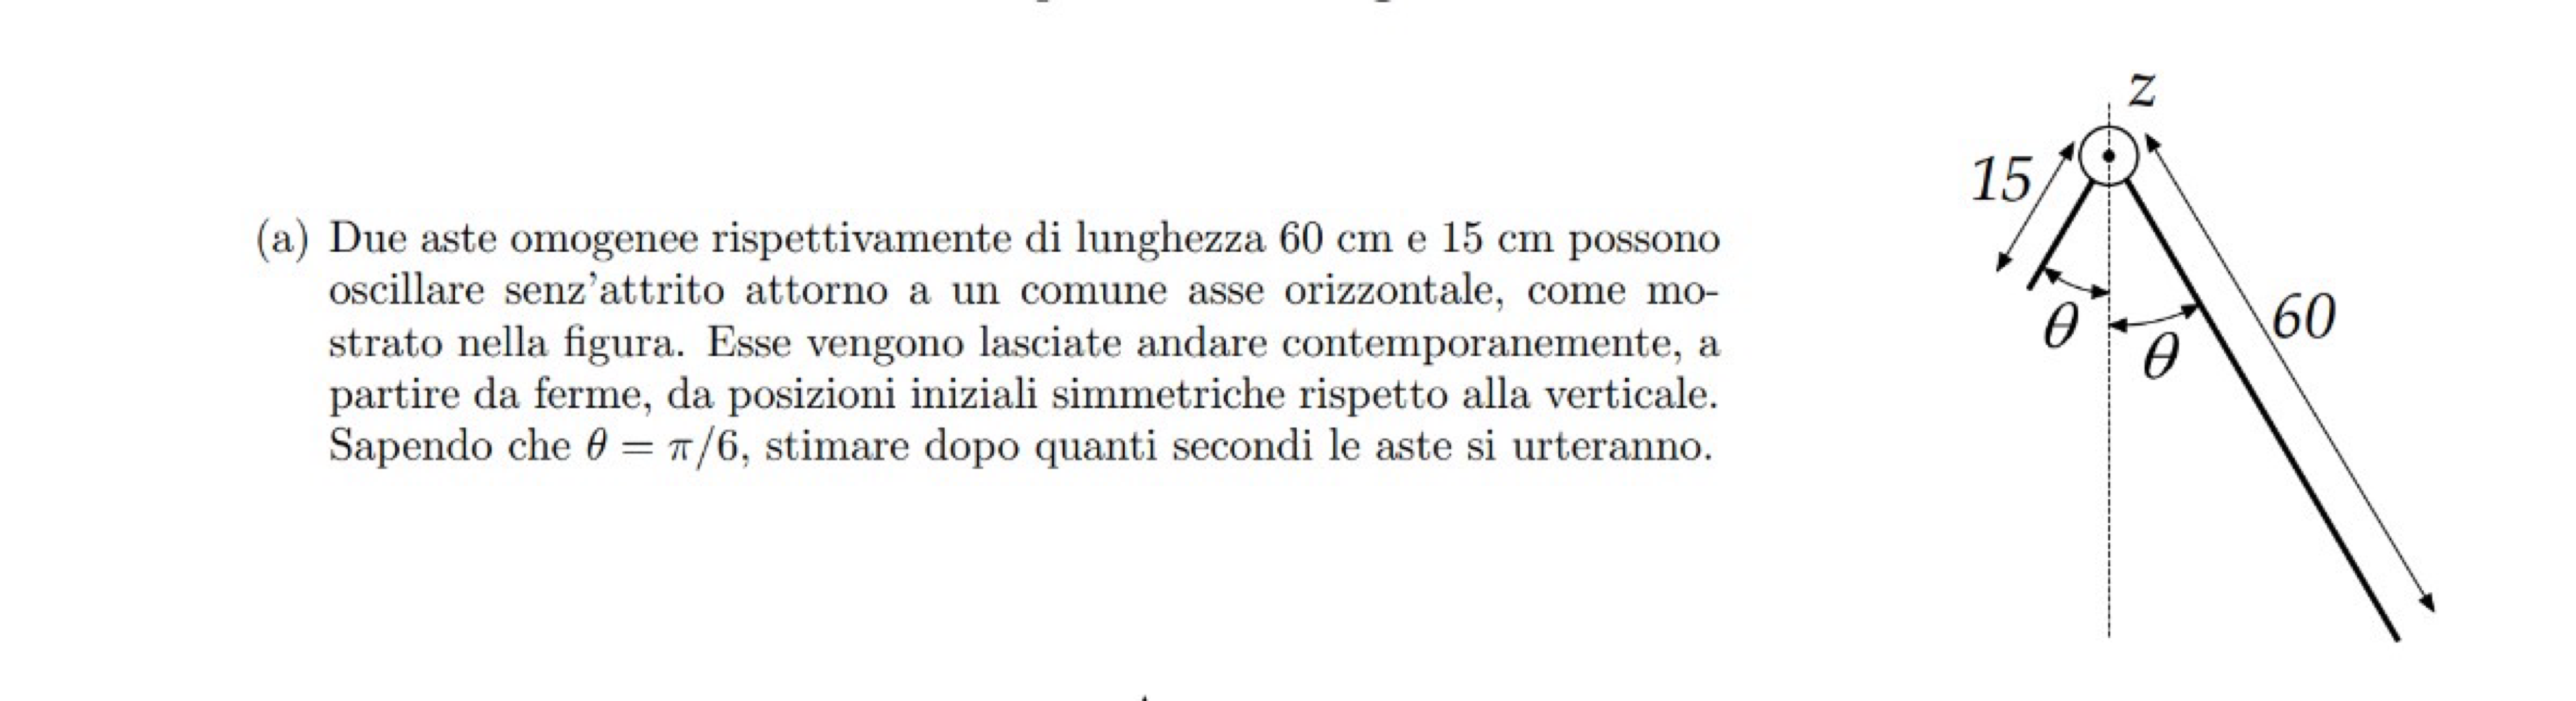
\includegraphics[width=0.9\linewidth]{EsercizioPiccoleOscillazioniPendoloSemplice.png}
    \label{fig:placeholder}
\end{figure}
\noindent
Vediamo ora come ragionare questo problema sulle piccole oscillazioni. \textbf{Il pendolo, effettua un moto armonico}. Per cui abbiamo rispettivamente due pendoli in questo esercizio che faranno un moto di questo tipo:
\begin{equation}
    \theta(t)=Asin(\omega t + \phi)
\end{equation}
I due pendoli si urteranno quando avranno lo stesso angolo. Per questo motivo l'idea è quella di eguagliare le leggi orarie. I due pendoli che d'ora in avanti chiameremo 1 quello di destra e 2 quello di sinistra, sono aperti dello stesso angolo per cui avranno ampiezza uguale che andremo a semplificare. Gli angoli invece che sono dati nel testo corrispondono alla fase iniziale, avremo quindi $\phi_1=\frac{\pi}{6}$ e $\phi_2=-\frac{\pi}{6}$. I dati rimanenti sono gli omega che troviamo facilmente in questo modo:
\begin{equation}
    \omega = \frac{2\pi}{T} \ \ \ \ \xrightarrow[]{T=2\pi\sqrt{\frac{l}{g}}} \ \ \ \ \omega=\sqrt{\frac{g}{l}}
\end{equation}
Per cui, eguaglio le due leggi orarie e mi esce un equazione con i seni.
\subsubsection{Come risolvere un'equazione con i seni}
Andiamo a mettere per quello con la fase negativa $+2K\pi$:
\begin{equation}
    sin(4t+\frac{\pi}{6})=sin(8t-\frac{\pi}{6})+2K\pi
\end{equation}
I seni sono uguali in due circostanze:
\begin{itemize}
    \item Il primo caso è quando gli \textbf{argomenti si eguagliano}:
    \begin{equation}
        4t+\frac{\pi}{6}=8t-\frac{\pi}{6}+2K\pi
    \end{equation}
    \item Il secondo caso è quando gli \textbf{angoli sono supplementari} (ovvero la loro somma è 180):
    \begin{equation}
        4t+\frac{\pi}{6}+8t-\frac{\pi}{6}=\pi+2K\pi
    \end{equation}
\end{itemize}
Impostando in entrambi i casi k=0 prendo come risultato la t minore.
\newpage
\section{Lezione 16}
\subsection{Introduzione}
Questa lezione è l'unione di due lezioni vedremo principalmente come affrontare le crocette e come affrontare problemi sui corpi rigidi tridimensionali.
\subsection{Crocette}
Vediamo diverse tipologie di crocette che non riguardano quella che è la teoria.
\begin{figure}[H]
    \centering
    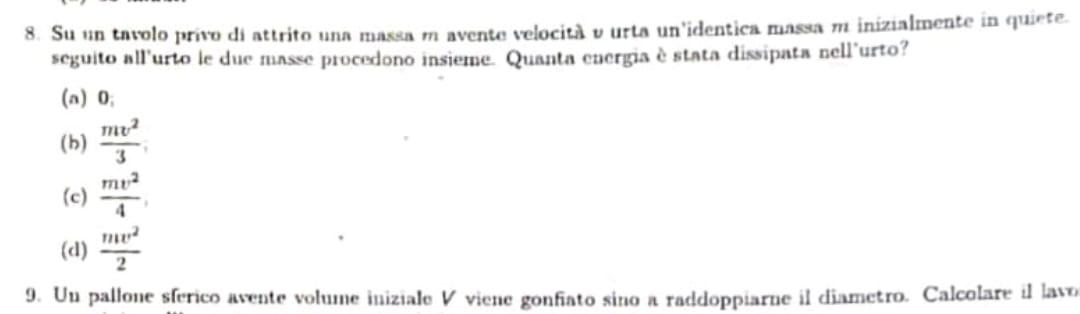
\includegraphics[width=0.9\linewidth]{CrocetteUrto.jpg}
    \label{fig:placeholder}
\end{figure}
\noindent
Per svolgere queste crocette è necessario capire il fenomeno fisico che sta avvenendo. Vuole sapere quant'è l'energia dissipata nell'urto e quindi per ottenerla dovremo sottrarre l'energia iniziale e quella finale.
\begin{equation}
    E_{M, iniziale}=E_k=\frac{1}{2}mv^2
\end{equation}
\begin{equation}
    E_{M,finale}=E_k=\frac{1}{2}2mv_f^2
\end{equation}
\begin{equation}
    mv_f^2-\frac{1}{2}mv^2=0
\end{equation}
Per trovare la velocità finale, sfrutto la quantità di moto:
\begin{equation}
    mv=2mv_f \xrightarrow[]{} v_f=\frac{v}{2}
\end{equation}
Sostituisco nell'equazione di prima:
\begin{equation}
    m\frac{v^2}{4}-\frac{v^2}{2}m = m\frac{v^2}{2}
\end{equation}
Vediamo ora delle crocette sulla gravitazione:
\begin{figure}[H]
    \centering
    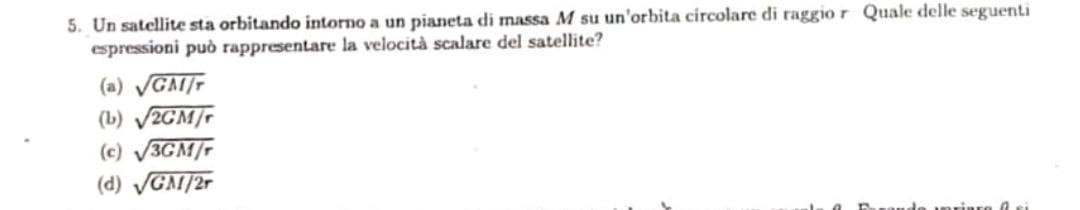
\includegraphics[width=0.9\linewidth]{CrocetteKeplero.jpg}
    \label{fig:placeholder}
\end{figure}
\noindent
Ogni satellite fa un'orbita circolare che rappresentiamo in questo modo:
\begin{figure}[H]
    \centering
    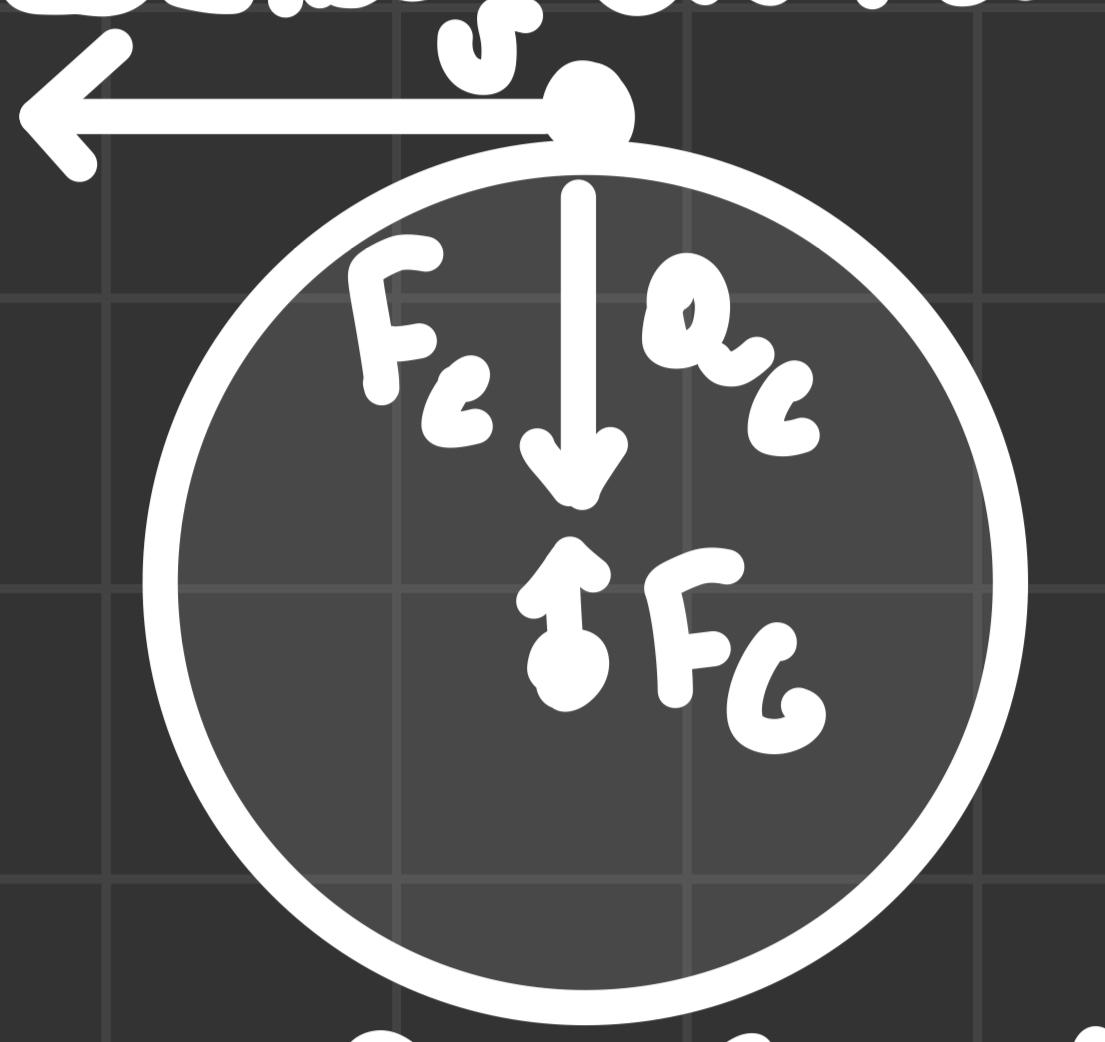
\includegraphics[width=0.3\linewidth]{orbitaSatellite.jpg}
    \label{fig:placeholder}
\end{figure}
\noindent
Dobbiamo fare un ragionamento simile a quello del giro della morte, dato che sta facendo un orbita circolare, ci sarà un accelerazione centripeta causata da qualcosa, questo qualcosa è la \textbf{forza gravitazionale}, se ho due masse a una certa distanza ho una certa forza attrattiva detta gravitazionale. Quindi:
\begin{equation}
    F_C=F_G \xrightarrow[]{} ma_C=\frac{G*m*M}{r^2}
\end{equation}
r è la \textbf{distanza tra i corpi} mentre G è la \textbf{costante gravitazionale universale}.
\begin{equation}
    m*\frac{v^2}{r}=\frac{G*m*M}{r^2} \xrightarrow[]{} v=\sqrt{\frac{G*M}{r}}
\end{equation}
\newpage
\begin{figure}[H]
    \centering
    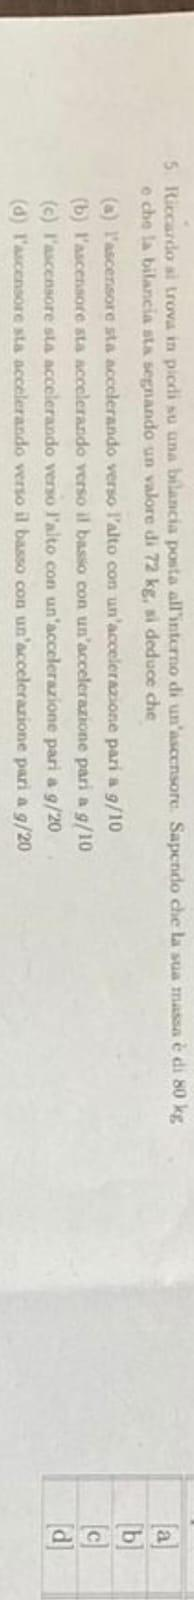
\includegraphics[width=0.2\linewidth, angle=90]{CrocetteAscensore.jpg}
    \label{fig:placeholder}
\end{figure}
\noindent
Intanto sappiamo che dato che la bilancia sta segnando un peso minore rispetto al peso reale l'ascensore sta accelerando verso il basso, questo perche in caso contrario, vi sarebbe una forza apparente che spingerebbe il corpo verso il basso, si dice quindi che siamo in un sistema non inerziale. Il problema parla di accelerazione e quindi sarà quello il focus principale. Considerando solamente la bilancia, questo perchè è l'unica che vede entrambe le forze in gioco applicate, disegnamo due forze la forza peso che va verso il basso e una forza apparente che spinge verso l alto e quindi ci fa avere quel risultato sulla bilancia. Avremo quindi che:
\begin{equation}
    P-F_A=P_F \xrightarrow[]{} mg-ma=ma_F \xrightarrow[]{} g-a=a_F
\end{equation}
Forza peso- forza apparente sarà uguale alla forza peso fittizia che vede la bilancia, di qui abbiamo due opportunità o ragioniamo risolvendo una proporzione: 
\begin{equation}
    80:9,8 = 72:x
\end{equation}
e troviamo quindi la $a_F$ accelerazione fittizia e risolviamo trovando a, oppure ragioniamo pensando che la bilancia è tarata per dare un certo peso con una accelerazione g e quindi (g/10)
\begin{equation}
    P_F=m*a_F \ \ \ \ oppure \ \ \ \ P_F = m_F * g
\end{equation}
eguagliamo risolviamo per $a_F$ e troviamo a.\\\\
Vediamo poi il quesito degli orologi che dice: Un orologio segna le tre. Le lancette dei minuti e delle ore si troveranno ad essere nuovamente ortogonali per la prima volta dopo circa: il trucco qui è quello di rappresentare l'orologio alle tre e banalmente vedere gli archi di tempo proposti e andare per esclusione. La risposta è \textbf{33 minuti}.
\begin{figure}[H]
    \centering
    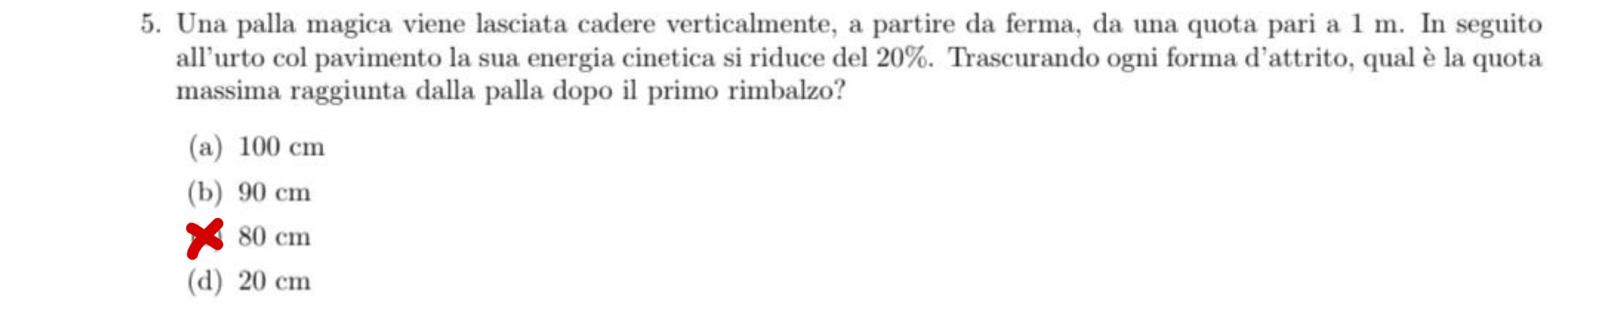
\includegraphics[width=0.9\linewidth]{CrocettaEnergia.jpg}
    \label{fig:placeholder}
\end{figure}
\noindent
Questo quesito si potrebbe ragionare con la conservazione dell'energia ma in realtà c'è un modo più intelligente, dato che l'energia meccanica rimane costante sapendo che l'energia dissipata è il 20$\%$ basta moltiplicare l'energia meccanica iniziale per $0.8$. Trovando $h=80cm$.
\begin{figure}[H]
    \centering
    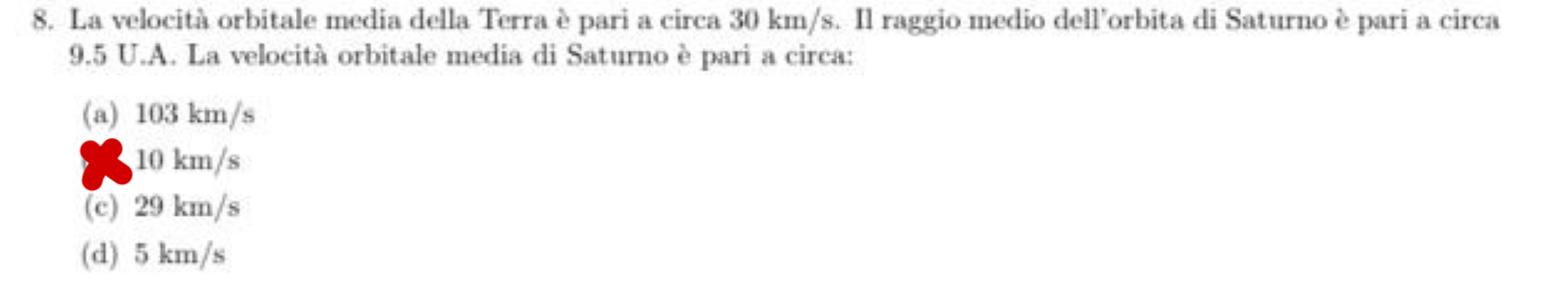
\includegraphics[width=0.9\linewidth]{Orbite.jpg}
    \label{fig:placeholder}
\end{figure}
\noindent
Per risolvere questo esercizio, è necessario conoscere la \textbf{terza legge di Keplero}. La quale ci dice che per ogni pianete rimane costante questo rapporto:
\begin{equation}
    \frac{T^2}{r^3}
\end{equation}
Dove T è il periodo orbitale del pianeta mentre r è il raggio dell'orbita. Ricordiamo inoltre che la velocità orbitale si trova come:
\begin{equation}
    v_{orb}=\frac{s}{T}
\end{equation}
Quindi possiamo impostare
\begin{equation}
    \frac{T_T^2}{R_T^3}=\frac{T_S^2}{R_S^3}
\end{equation}
Bisogna ricordare inoltre che 1 unità astronomica sarebbe la distanza tra la terra e il sole, quindi sappiamo anche il raggio della terra. Impostiamo
\begin{equation}
    \frac{T_T^2}{UA^3}=\frac{T_S^2}{(9,5UA)^3} \xrightarrow[]{} T_T^2=\frac{T_S^2}{857}=T_T=\frac{T_S}{29}
\end{equation}
Una metodologia utile alla risoluzione delle crocette è quella di fare il rapporto tra due equazioni, in particolare:
\begin{equation}
    V_{orb,saturno}=\frac{s}{T}=\frac{2\pi R_{saturno}}{T_{saturno}}
\end{equation}
\begin{equation}
    V_{orb,terra}=\frac{s}{T}=\frac{2\pi R_{terra}}{T_{terra}}
\end{equation}
Ne faccio il rapporto e trovo la velocità orbitale di saturno. Questo rapporto mi è utile perchè mi permette di utilizzare il rapporto che ho precedentemente trovato.
\newpage
\begin{figure}[H]
    \centering
    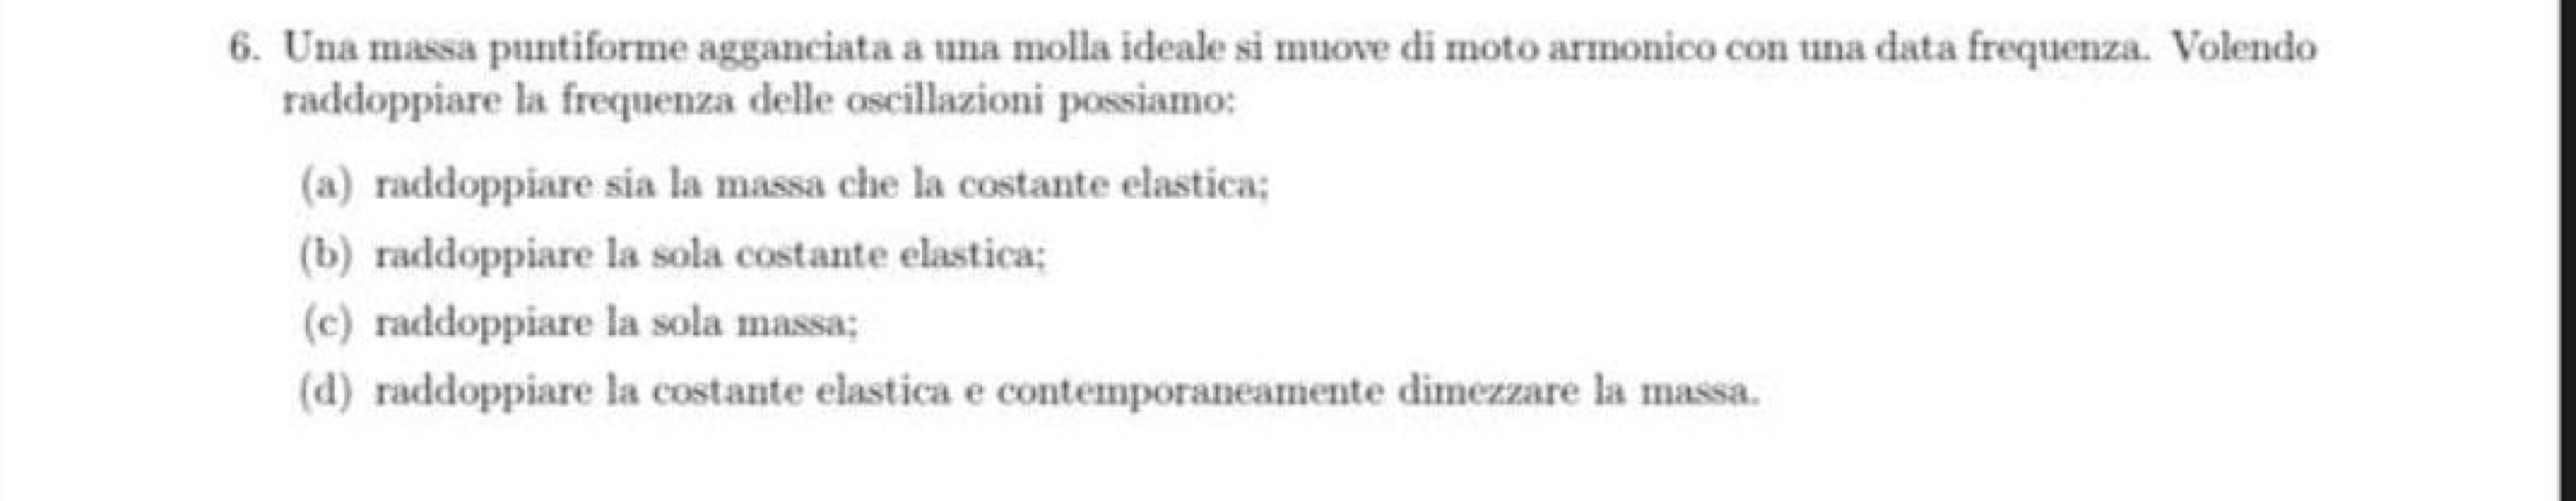
\includegraphics[width=0.9\linewidth]{CrocetteFrequenza.png}
    \label{fig:placeholder}
\end{figure}
\noindent
Per fare quest'esercizio basta semplicemente vedere la formula della frequenza:
\begin{equation}
    f=2\pi \sqrt{\frac{k}{m}}
\end{equation}
\begin{figure}[H]
    \centering
    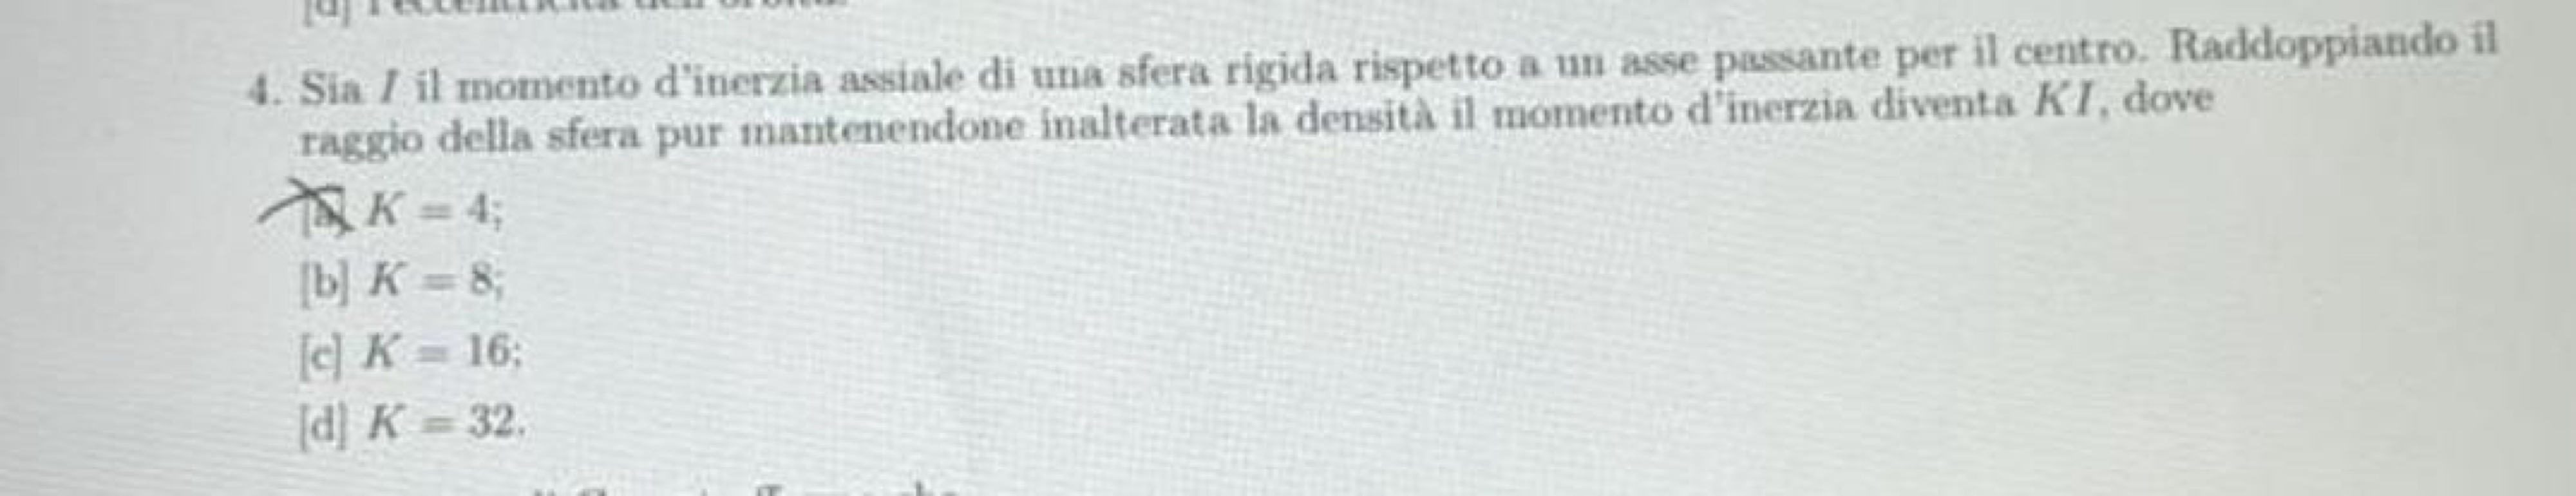
\includegraphics[width=0.9\linewidth]{CrocettaMomentoD'Inerzia.png}
    \label{fig:placeholder}
\end{figure}
\noindent
Per risolvere quest'esercizio è necessario pensare a quello che ci dice il testo, partiamo dal momento d'inerzia della sfera:
\begin{equation}
    I=\frac{2}{5}mr^2
\end{equation}
Successivamente parla di densità, la cui formula:
\begin{equation}
    d=\frac{m}{V}
\end{equation}
Dove V è il volume che per la sfera è: $\frac{4}{3}\pi r^3$. Di conseguenza calcolo la massa in funzione della densità, sostituisco nel momento d'inerzia e impongo $r=2r$. Risposta 32.
\begin{figure}[H]
    \centering
    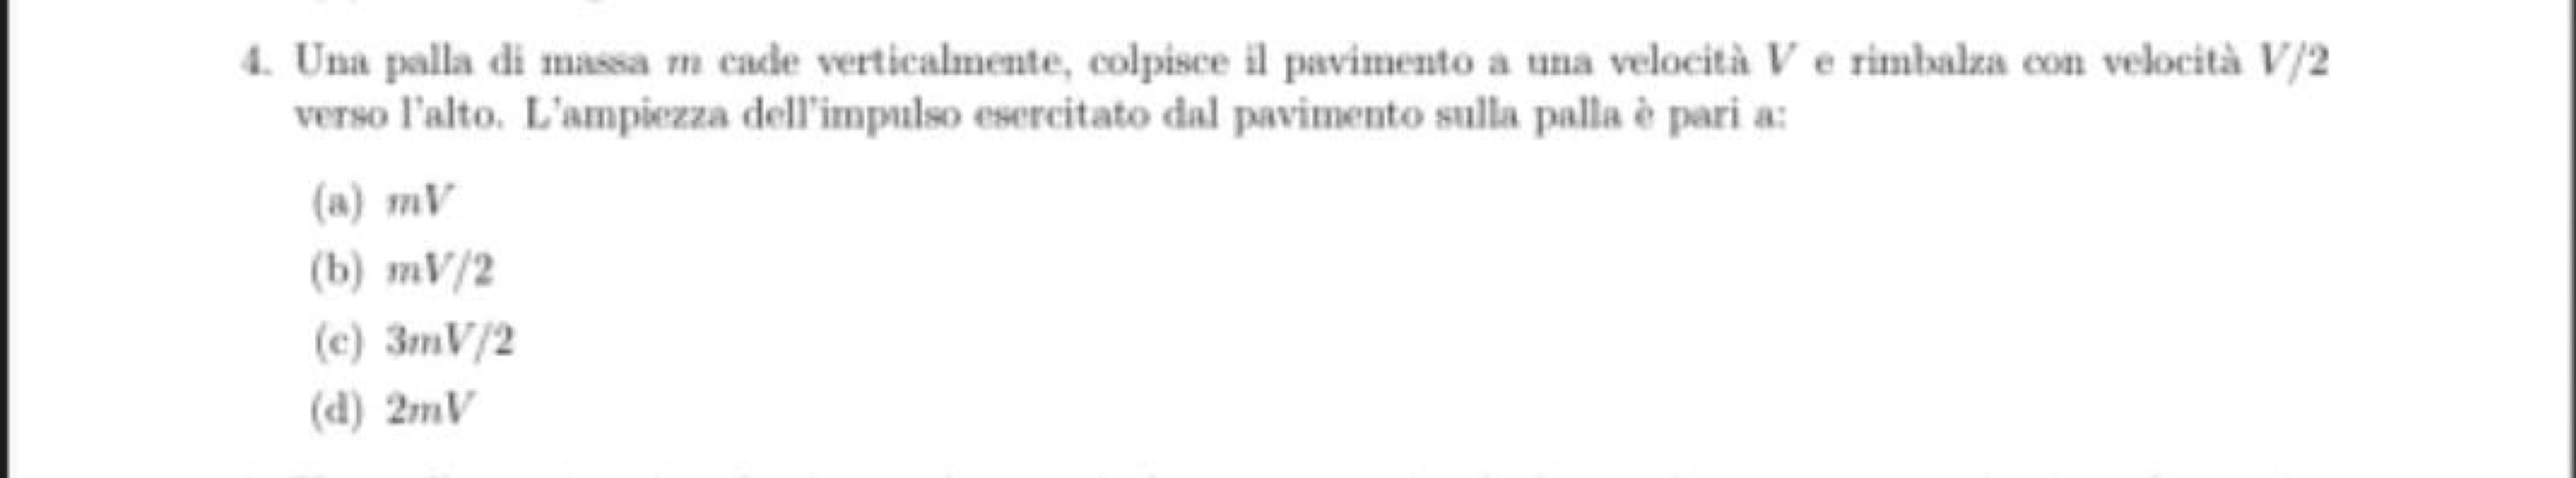
\includegraphics[width=0.5\linewidth]{CrocetteImpulso.png}
    \label{fig:placeholder}
\end{figure}
\noindent
Siccome sappiamo che l'impulso è uguale alla variazione della quantità di moto, ricordando che è un equazione vettoriale e quindi la quantità di moto iniziale è presa negativa:
\begin{equation}
    q_F-q_I=J \xrightarrow[]{} m\frac{V}{2}-(-mV)=J\xrightarrow[]{} J=\frac{3mV}{2}
\end{equation}
\begin{figure}[H]
    \centering
    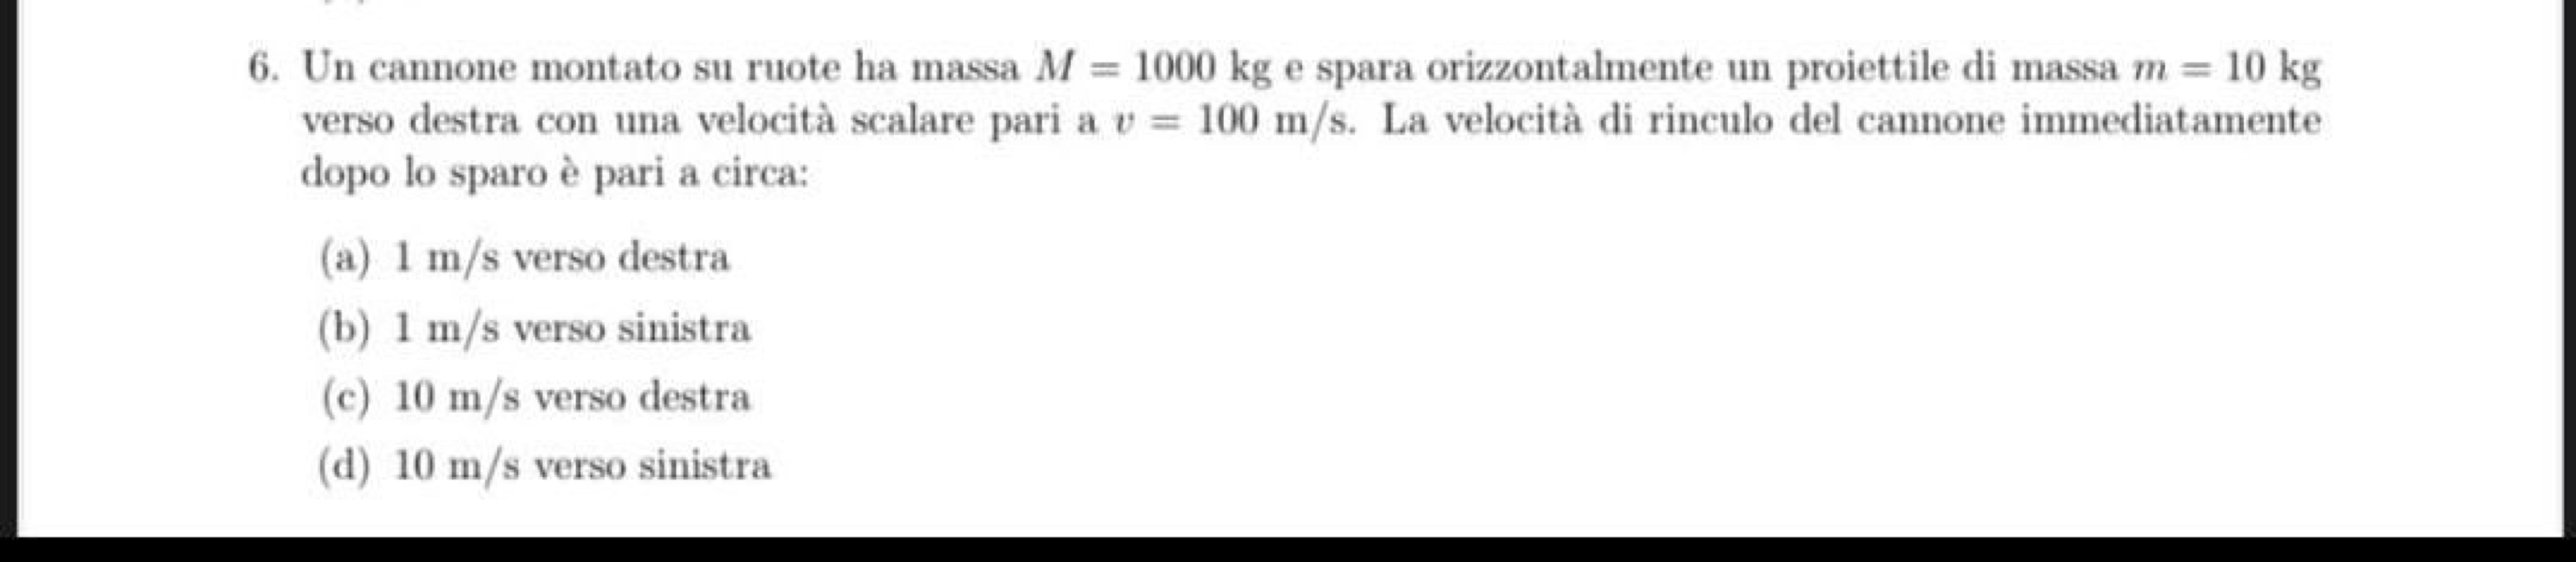
\includegraphics[width=0.9\linewidth]{CrocettaCannone.png}
    \label{fig:placeholder}
\end{figure}
\noindent
Innanzitutto la velocità è di rinculo e quindi deve andare nel verso opposto rispetto al proiettile, detto questo il fenomeno va inteso come un urto anelastico in cui i due inizialmente sono entrambi fermi:
\begin{equation}
    0=m_Pv_P-m_Cv_C \xrightarrow[]{}v_C=\frac{m_Pv_P}{m_C}=1 m/s
\end{equation}
\begin{figure}[H]
    \centering
    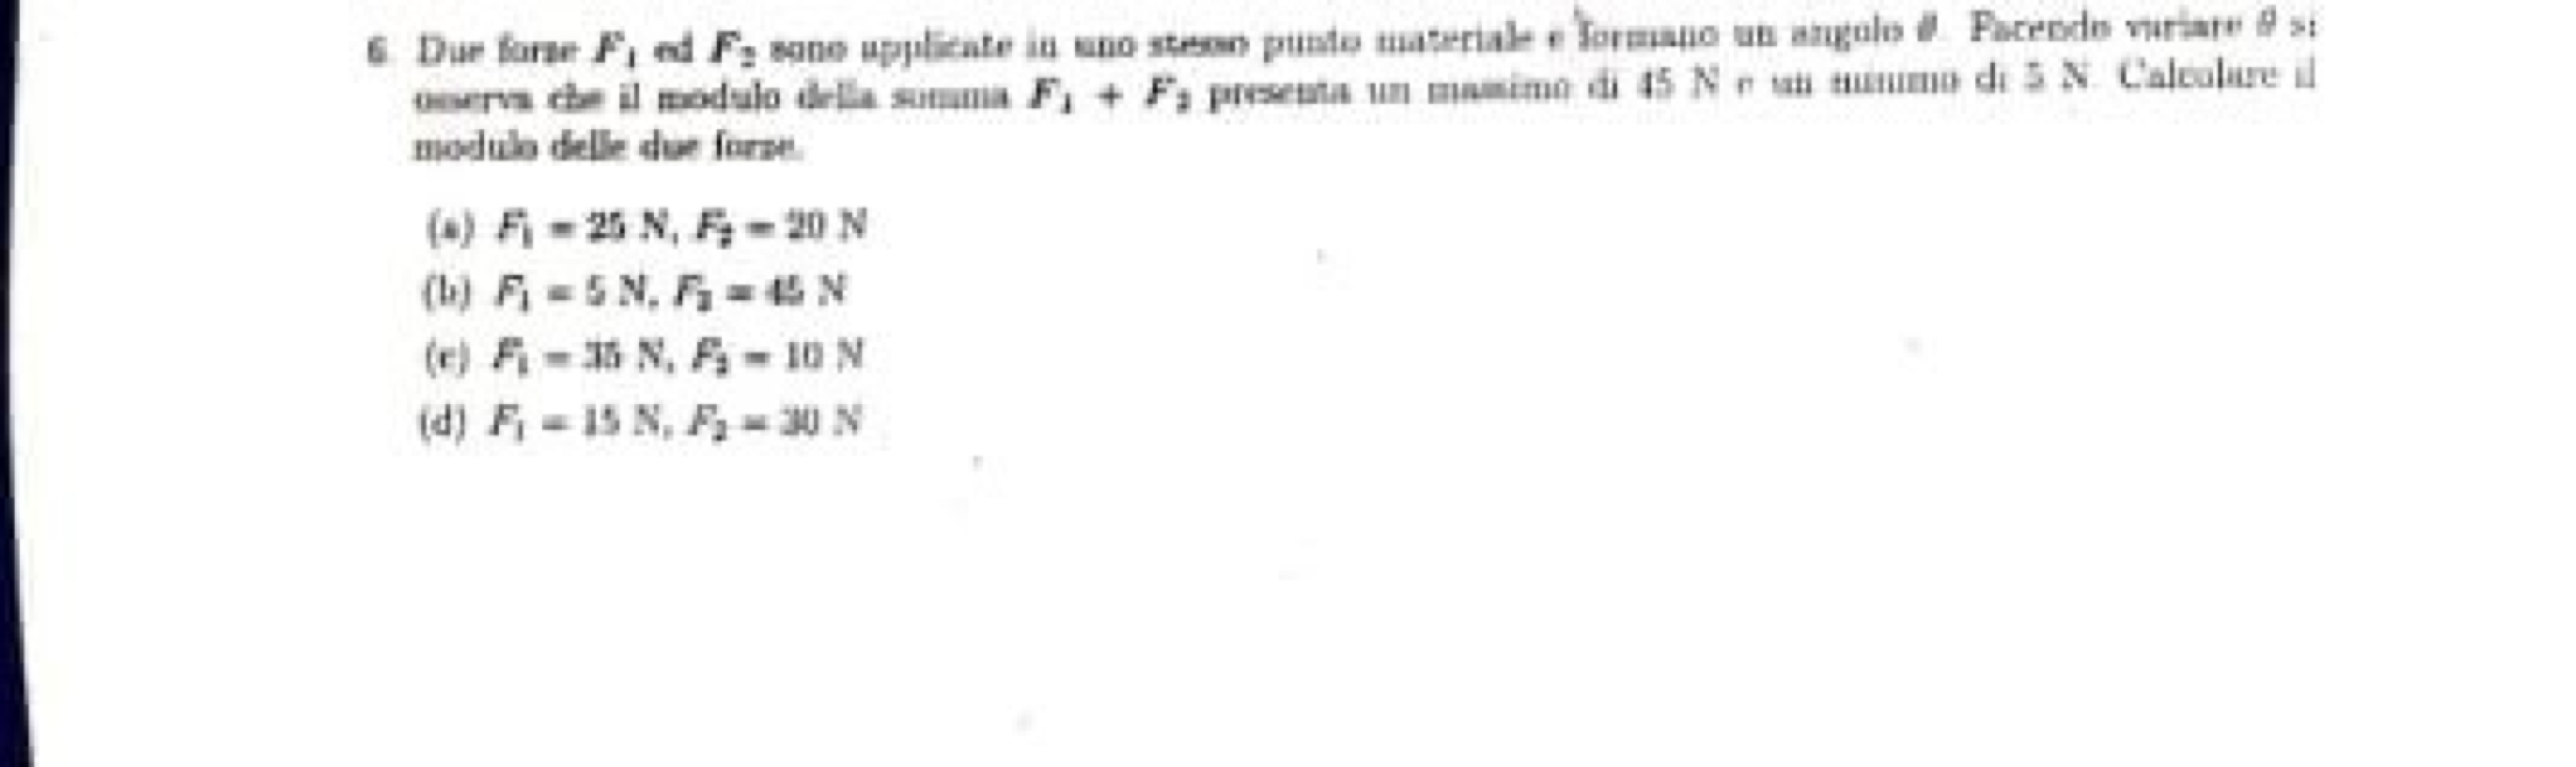
\includegraphics[width=0.9\linewidth]{CrocetteVettori.png}
    \label{fig:placeholder}
\end{figure}
\noindent
Questo problema, è in realtà un problema di natura vettoriale, infatti \textbf{due vettori ottengono il massimo della somma quando sono concordi} mentre \textbf{il minimo quando sono discordi} quindi:
\begin{equation}
    F_1+F_2=45
\end{equation}
\begin{equation}
    F_1-F_2=5
\end{equation}
Risolvo.\\
\newpage
\subsection{Crocette sui vettori}
Per quanto riguarda le nozioni sui vettori, le cose principali da conoscere sono:
\subsubsection{Prodotto Scalare}
\begin{equation}
    a \cdot b
\end{equation}
Ci da come risultato uno scalare. Si calcola come:
\begin{equation}
    |a| * |b| * cos(\alpha)
\end{equation}
Dove alpha è l'angolo formato tra i due. Di conseguenza a determinare il massimo e il minimo è il coseno. Sarà il \textbf{minimo} quando i vettori sono paralleli ($cos(180)=-1$) e hanno verso opposto sarà \textbf{massimo} quando i vettori sono paralleli e hanno stesso verso ($cos(0)=1$) e sarà 0 quando sono ortogonali ($cos(90)=0$).
\subsubsection{Prodotto Vettoriale}
\begin{equation}
    a \times b
\end{equation}
\begin{figure}[H]
    \centering
    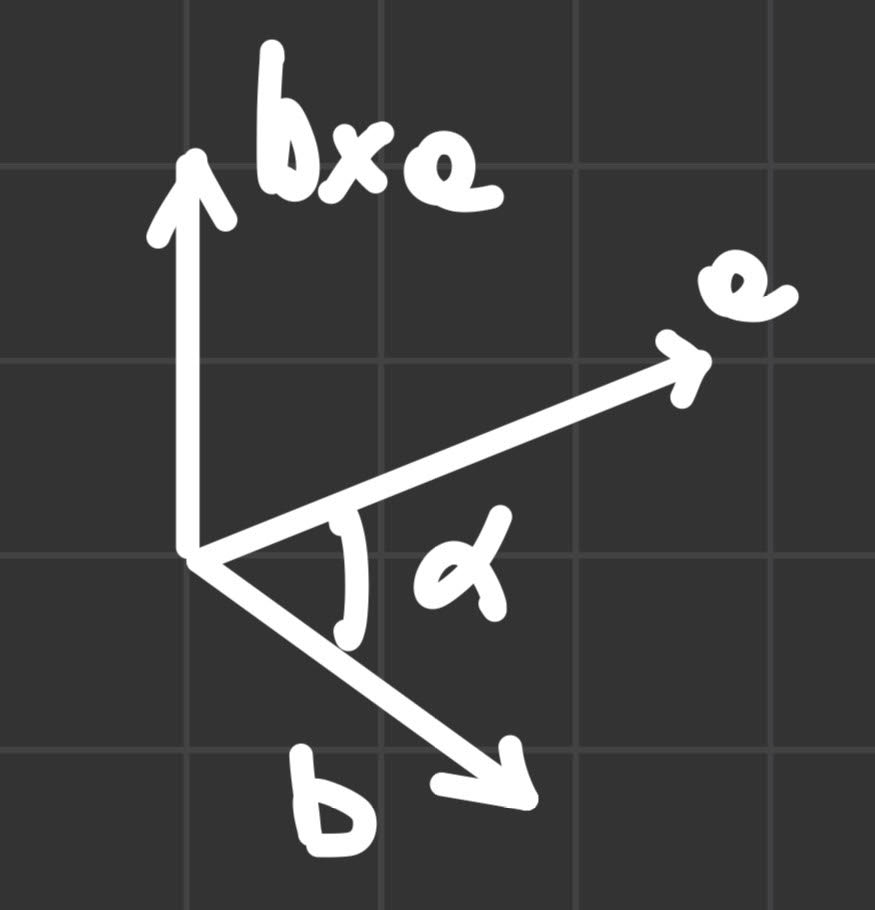
\includegraphics[width=0.3\linewidth]{ProdottoVettoriale.jpg}
    \label{fig:placeholder}
\end{figure}
\noindent
Ci da come risultato un vettore, generalmente le domande sono relative al modulo:
\begin{equation}
    |a \times b| = |a| * |b| * sin(\alpha)
\end{equation}
Di conseguenza, è massimo quando sono ortogonali ($\sin (90)=1$), 0 quando sono paralleli ($sin(0)=0$) e minimo quando sono ortogonali "al contrario" ($sin(270)=-1$).
\subsubsection{Regola della manodestra}
Per capire da un disegno se è $a \times b$ o $b \times a$ bisogna utilizzare la regola della manodestra. Se abbiamo a verso sinistra, b andrà verso l'esterno e il risultato verso il basso. Se a va verso sinistra, b andrà verso l'esterno e il risultato verso l'alto.
\subsubsection{Terne}
Inoltre ricordiamo che dei vettori che sono perpendicolari agli assi cartesiani li chiamiamo \textbf{terna destrogira} al contrario \textbf{terna sinistrogira}. Geometricamente $a \times b$ rappresenta l'area di un parallelogramma.
\subsection{Corpo rigido tridimensionale}
Importante notare come gli esercizi tridimensionali riguardanti il corpo rigido per risolverli basta riportarli come bidimensionali.
\subsection{Nota su termodinamica}
In un esercizio in cui è presente un cilindro con pareti adiabatiche e un pistone esposto alla sola pressione esterna 1 atm potrebbe esserci una richiesta del tipo: "si porta velocemente la pressione al doppio di quella iniziale" questo vuole dire che parliamo di una trasformazione \textbf{irreversibile}. Notare inoltre come se raddoppiamo la pressione significa che stiamo comprimendo il gas e quindi nel piano PV il punto finale sarà dietro al punto iniziale. Si puo considerare la trasformazione in questo modo, nonostante l'area sia sempre quella del trapezio, considerando la finale e iniziale invertite:
\begin{figure}[H]
    \centering
    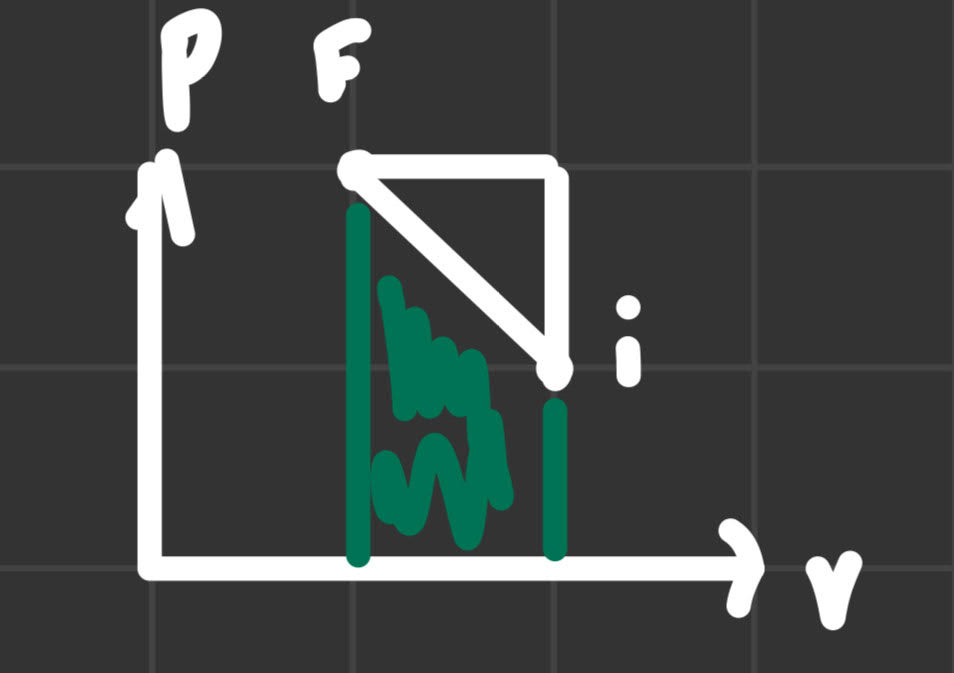
\includegraphics[width=0.5\linewidth]{TrasformazioneIrreversibile.jpg}
    \label{fig:placeholder}
\end{figure}
\noindent
Infatti quello che succede è che consideriamo il gas che avendo subito una pressione molto velocemente, inizialmente non riesce a comprimersi e quindi compie una trasformazione isocora, successivamente passa a 2 atm e quindi subisce una trasformazione isobara fino alla fine, unisco i due punti e l'area sottesa è la solita del trapezio.
\clearpage
\end{document}
